% mainfile:main.tex
\synctex=1

\documentclass[a4paper,11pt,twoside]{book}

\usepackage[pdftex]{graphicx}
\usepackage{fancyhdr} % for the headers
\usepackage[Lenny]{fncychap}
\usepackage{eurosym} % for the euro symbol
\usepackage[pagebackref=true]{hyperref} % for hyperlinks
\usepackage{setspace} % margin configuration
\usepackage{url}
\usepackage{wrapfig}
\usepackage{tabularx}
\usepackage{float}
\usepackage{tocbibind} % to show the bibliography in the index

\hypersetup{
    unicode=false,
    pdftoolbar=true,
    pdfmenubar=true,
    pdffitwindow=false,
    pdfstartview={FitH},
    pdftitle={Road to gedit 3.0},
    pdfauthor={Ignacio Casal Quinteiro},
    pdfsubject={},
    pdfcreator={},
    pdfproducer={},
    pdfkeywords={},
    pdfnewwindow=true,
    colorlinks=true,
    linkcolor=blue,
    citecolor=green,
    filecolor=magenta,
    urlcolor=blue
}

\usepackage{color}
\definecolor{gray97}{gray}{.97}
\definecolor{gray75}{gray}{.75}
\definecolor{gray45}{gray}{.45}

\usepackage{listings}
\lstset{
  frame=Ltb,
  framerule=0pt,
  aboveskip=0.5cm,
  framextopmargin=2.5pt,
  framexbottommargin=2.5pt,
  framexleftmargin=0.4cm,
  framesep=0pt,
  rulesep=.4pt,
  backgroundcolor=\color{gray97},
  rulesepcolor=\color{black},
  tabsize=8,
  %
  stringstyle=\ttfamily,
  showstringspaces = false,
  basicstyle=\small\ttfamily,
  commentstyle=\color{gray45},
  keywordstyle=\bf,
  %
  numbers=left,
  numbersep=15pt,
  numberstyle=\tiny,
  numberfirstline = false,
  breaklines=true
}

% minimize the fragmentation
\lstnewenvironment{listing}[1][]{
  \lstset{#1}\pagebreak[0]}{\pagebreak[0]
}

\lstdefinestyle{GObject}{
  language=C,
  emph={gboolean, gpointer, gconstpointer, gchar, guchar, gint, guint, gshort,
        gushort, glong, gulong, gfloat, gdouble, gsize, gssize, goffset},
  emphstyle=\color{blue}
}

\lstdefinestyle{python}{
  language=python
}

\lstdefinestyle{xml}{
  language=XML
}

\lstdefinestyle{plain}{}

% override the title setting to make it bold
\ChTitleVar{\bf\Huge}

% margin configuration
\onehalfspacing
\setlength\textwidth{15cm}
\setlength\textheight{22cm}
\setlength\oddsidemargin{0.2cm}
\setlength\evensidemargin{0.2cm}

\parskip=6pt
\parindent=10pt

\author{Ignacio Casal Quinteiro}
\title{\textbf{\Huge{Road to gedit 3.0}}}

\begin{document}

%==============================================================
% Custom commands
%==============================================================

% addwrapfigure
\newcommand{\addwrapfigure}[4][\textwidth]{
  \begin{wrapfigure}{#2}{#1}
    \vspace{-20pt}
    \begin{center}
      \includegraphics[width=#1]{#3}
    \end{center}
    \vspace{-20pt}
    \caption{#4}
    \vspace{-20pt}
  \end{wrapfigure}
}

\newcommand{\addfigure}[4][width=\textwidth]{
  \begin{figure}[H]
    \begin{center}
      \includegraphics[#1]{#2}
      \caption[#3]{#3}\label{#4}
    \end{center}
  \end{figure}
}

% make GNOME prettier
\newcommand{\GNOME}{\textsc{Gnome}~}

% graybox
\newcommand{\graybox}[1]{\colorbox{gray75}{#1}}

%===============================================================
%Title
%===============================================================
% mainfile:main.tex

\begin{titlepage}

\begin{center}

% Upper part of the page

\textsc{\Huge Road to gedit 3.0}\\[2.0cm]


\includegraphics[scale=0.8]{./images/uvigo}\\

\vfill

% Author and supervisor
\begin{tabularx}{\linewidth}{lXl}
  \emph{Author:} && \emph{Supervisor:} \\
  Ignacio \textsc{Casal Quinteiro} && Dr.~David \textsc{Olivieri}
\end{tabularx}

\end{center}

\end{titlepage}

\newpage\thispagestyle{empty}
\cleardoublepage

%===============================================================
% Dedication
%===============================================================
% mainfile:main.tex

\chapter*{}

\begin{flushright}
  \textit{
    To my family for all the support given all these years.\\
    No words can show how thankful I am to them.
  }
\end{flushright}

\newpage\thispagestyle{empty}
\cleardoublepage

%===============================================================
% For the headers
%===============================================================
\pagestyle{fancy}
\fancyhf{}
\fancyhf[HR]{\thepage}
\fancyhf[HL]{\nouppercase\rightmark}

%===============================================================
%Index
%===============================================================
\frontmatter

\tableofcontents
\listoffigures
\listoftables
\newpage\thispagestyle{empty}
\cleardoublepage

%===============================================================
% Chapters
%===============================================================
\mainmatter

\part{Memory}
% mainfile:main.tex

\chapter{Project Identification}

\textbf{Title:} \textsc{Road to gedit 3.0}\\
\textbf{Code:} %FIXME put he code here

\noindent\textbf{Author:} Ignacio \textsc{Casal Quinteiro}\\
\textbf{ID number:} \\ % FIXME: not for now
\textbf{Date:} \today

\noindent\textbf{Supervisor:} David \textsc{Olivieri}\\
\textbf{Area:} Languages and Informatic Systems\\
\textbf{Department:} Computer Engineer

% mainfile:main.tex

\chapter{Introduction}

The \GNOME Project was started in 1997 by two then university students, Miguel de Icaza and Federico Mena. Their aim: to produce a free (as in freedom) desktop environment. Since then, \GNOME has grown into a hugely successful enterprise. Used by millions of people across the world, it is the most popular desktop environment for GNU/Linux and UNIX-type operating systems. The desktop has been utilised in successful, large-scale enterprise and public deployments, and the project’s developer technologies are utilised in a large number of popular mobile devices\cite{website:gnome}.

Since the project has started, \emph{gedit} has been the default text editor. As part of \GNOME this program must be up to date, evolving with the desktop. The \GNOME comunity is the one that defines the schedules between versions for each program and also sets which libraries fit the standards to be used by the applications, or which libraries should get deprecated.

With this project it is proposed to add new features to \emph{gedit} and develop it from the version 2.30 to the version 3.0 in the way of using this new technologies (see page \pageref{chap:Technologies}).

% mainfile:main.tex

\chapter{Objectives of the project}

% FIXME: draft

The objective it is to increase the the functionality of \emph{gedit} by adding new features and by porting it to the new libraries needed to be part of \emph{\GNOME 3}.

% mainfile:../main.tex

\section{Port to new libraries}\label{sec:NewLibraries}

\subsection{GTK+ 3}\label{sec:GTK3}

Migrate from GTK+ 2 to GTK+ 3. This will mean to get rid of deprecated code that it is used from GTK+ 2, update gedit to use the new APIs and the most important thing, follow the development of GTK+ 3, meaning that if there is any error in GTK+, it should be filed a bug against it and if possible provide a patch to fix it (See \ref{sec:Patches} for an explanation on how it is done correctly). This will also mean that to have the application building, it will be needed to have the application up to date, which will mean a lot of testing against the latest libraries and rebuilding them. For an explanation of what GTK+ is, see the section \ref{sec:GTK}.

\subsection[GSettings]{GSettings\cite{website:gio}}\label{sec:GSettings}

Port to GSettings, to use it instead of GConf. GSettings is part of glib (see \ref{sec:GLib}) and provides a convenient API for storing and retrieving application settings. Some of the reasons for this switch are:
\begin{itemize}
  \item GConf has been deprecated.
  \item Provides better API to be used by GObject-based applications.
  \item It is used over DBus.
  \item The storage system is implemented by different backends, in relation to the operative system or the choose of the user.
\end{itemize}

\subsection{libpeas}\label{sec:libpeas}

Remove custom plugin system and use libpeas instead. See the section \ref{sec:peas} for a better explanation of what libpeas is.

\subsection{GObject-introspection}\label{sec:GObjectIntrospection}

It will allow to remove the static bindings and generate dynamic ones by making annotations in the public API of \emph{gedit}. See \ref{sec:g-i} for a better explanation of what GObject-introspection is.

% mainfile:../main.tex

\section{New features}\label{sec:NewFeatures}

Besides the major library changes provided by this project, that are hidden from the 
user, there are several more visible changes undertaken in this project, that have been 
realized.  Each of the major feature changes is described below.


\subsection{Remove old API}\label{sec:RemoveOldAPI}

For several years, developers of \emph{gedit} have opted for maintaining a stable unchanging 
API interface for plugin- developers. The implication of this cautious design choice in the 
evolution of \emph{gedit} has been a continual growth in deprecated and duplicated code 
in order to lessen the burden of plugin developers need to update to the new API features. 
Thus, if some part of the API was deprecated, it would be marked as such, yet maintained 
in the source tree, still available to third party plugins, without the need for update action.
A result of such a policy is .....

The objectives of this project for providing a major release of \emph{gedit}, removes 
all references to the old API.  Thus, several older plugins will cease to be supported 
unless updated.


\subsection{New highlighting language files}\label{sec:HighFiles}

A new feature, provided by software written for this project, is the use of 
highlighting language files.   Since it is common to receive requests from 
users for highlighting for new programming files, (....why?? )

Thus, this project has added the use of this feature, to fix, review and 
add new language files to highlight syntax for new programming languages.


\subsection{Tab Groups}\label{sec:TabGroups}

An important editor feature, that is clearly desirable in a full feature application 
such as \emph{gedit}, is to be able to edit multiple documents side-by-side. 
Such a feature is useful for comparison, and is common in applications such as emacs. 
Thus, this feature has been added as a design objective for this project.


\subsection{Manage invalid characters}\label{sec:InvalidChars}



GTK+ is UTF-8\footnote{UTF-8 is a multibyte character encoding for Unicode.} oriented. There 
are several characters\footnote{An invalid byte sequence is a sequence of bytes that can not be 
together in an UTF-8 encoded system.} in UTF-8 that cannot be introduced in GTK+ widgets. 
In \emph{gedit} the documents that contain invalid characters are treated as binary files and not 
opened, this is sometimes not good when you have a wrongly encoded document and you want to fix it. 
This feature will allow to open this kind of documents.

\subsection{Use new Drag and Drop system}\label{sec:DND}

The present stable version of \emph{gedit} uses a custom implementation to make 
drag and drop of opened tabs.  Given that the new GTK+ supports all the functionalities 
needed by gedit, the custom drag/drop code is no longer required and should take advantage
of the more robust GTK+ API.  Moreover, the GTK+ API allows for better integration 
with the desktop and provides for a cleaner implementation of the \emph{gedit} source code.
As such, this is a major feature contribution provided by this project. 

\subsection{New search system}\label{sec:SearchSystem}

The present method that \emph{gedit} searches files is obsolete and does not take advantage of 
the latest algorithms nor graphical user interface philosophies, such as embedding the search 
entry in the bottom of the window (as Firefox) or sliding out the search entry (as with Chrome). 
Instead, the \emph{gedit} has used a dialog for searching, with all its associated problems. 

An important contribution of this project has been to change the manner of searching text 
within documents.


% mainfile:main.tex
% revised by dnolivieri
\chapter{Technical description}


Despite the apparent simplicity of the \emph{gedit} application for the end user, it 
is actually a highly complex software system, having its special idiosyncratic 
architectural solutions.   Before describing the actual work of this project, a brief 
description of the \emph{gedit} architecture shall be discussed, so as to better appreciate 
the work involved in the upgrade.


\section{Gedit Architecture}

The \emph{gedit} application is written in the \emph{C} language and built around the 
GObject paradigm, invented by \GNOME, and thereby endowing the language with object-oriented constructs. 
Figure \ref{fig:geditArch} shows a simple architectural overview of the \emph{gedit} internals.

\addfigure[width=0.60\textwidth]{./images/old-architecture}{gedit architecture}{fig:geditArch}

\paragraph{GConf}

The facto standard for GObject applications to store its settings in a database 
providing applications with a signal system to detect whether a specific setting 
has been modified externally, allowing to the application to adapt itself to the 
change. This helped \GNOME applications to be simple in relation to the user interface, 
not providing too many options, but giving the possibility to change advanced options 
externally from the GConf database with its utility \emph{gconf-editor}.
GConf has become deprecated and one major change for the Project is to remove 
this dependency on the architecture, as right now all the settings are intrinsic 
in all parts of \emph{gedit}.

\paragraph{GLib}

GLib provides data structure handling for C, portability wrappers, and interfaces 
for such runtime functionality as an event loop, threads, dynamic loading, and an object 
system. It is the main reason gedit is written in \emph{C} as it has been the 
promoted language by the platform and ten years ago the only supported language 
by \GNOME. See section \ref{sec:GLib} for more information about this library.

\paragraph{Cairo}

Cairo is a 2D graphics library designed to produce consistent output on all output 
media while taking advantage of display hardware acceleration when available. It 
has a direct used by the GTK+ library and applications like gedit using GTK+.

\paragraph{GTK+}

Multi-platform toolkit used in \emph{gedit} which allows to create graphical interfaces.
The architecture is totally tied up to this library, as gedit makes direct use of its 
API in the core. The fact that we depend directly on its API it means that gedit 
needs a lot of work in order to work with the new features and changes provided 
on this library and in some cases modify and fix the library to make it work correctly 
for gedit. See section \ref{sec:GTK} for more information about GTK+.

\paragraph{GtkSourceView}

GtkSourceView is a library maintained by the \emph{gedit team} which extends the main 
multiline text editing widget. It features syntax highlighting, completion framework, 
line marks... In general what a source editor needs. Gedit makes use of this library 
and it is tied to it architecturally and in the design. Part of the project gets some 
focus on this library.

\paragraph{gedit}

This is the core. Where the project take more focus and where most of the modification 
are made. Parts of the core are explained in the Project in farther sections of this 
document.

\paragraph{Plugins}

\emph{gedit} emphasizes simplicity but it can be also extended in a powerful way 
by plugins. Figure \ref{fig:pluginsArch} shows in a really simplistic way how plugins 
are tied up in an architectural way.

\addfigure[width=0.60\textwidth]{./images/old-plugins-architecture}{gedit plugins architecture}{fig:pluginsArch}

We can see that they make direct use of static python bindings, being very attached 
to them. With the GObject-introspection work this layer is removed, making use of a 
slightly different API provided by the dynamic bindings. This project shows how it has 
been done and the amount of work required.


\section{Programming languages used in Project}
\label{sec:ProgrammingLanguages}

Before describing the exact technical contribution of the project, it is useful to briefly mention 
the programming languages and tools that were needed.  

\paragraph{C}

The \emph{C} programming language is used in the core of \emph{gedit}.   As such, it is 
the recommended language of choice for the platform.  By using GObjects, several 
object oriented features are exposed to the developer.  Apart from the technical advantages, 
these features greatly aide the organization as well as readablility of the code.
All upgrades that were carried out were written in the \emph{C} language with explicit
use of the GObjects paradigm. 

\paragraph{Python}

Python is a powerful object oriented interpreted language that provides powerful 
C- level bindings, and is not only useful as a stand-alone language but can be used 
as a plugin - development language, for its ease of use.   By wrapping the core 
C API, plugin development in python is fast, easy to develop and maintain, and 
can avoids the heavy learning curve associated with the low-level C programming 
associated with \emph{gedit}.

Python has been used in this project mainly to develop and update the powerful 
plugins provided by \emph{gedit}. It has been also used to provide the specific 
unit tests and overrides into pygobject in order to get new functionalities needed by 
\emph{gedit} plugins. The overrides are methods or classes that from a direct 
bind from C to Python do not result as convenient as they should and by adding 
overrides the powerful of Python can be used in advantage by for example converting
some specific classes in iterated classes.


\paragraph{Tools and Formats}


An important part of the development for an open-source project such as \emph{gedit} is 
the use of complex build tools.   For this, Autotools is used. 
Together with the Makefile utilities, the Autotools suite are used for creating complex
compile dependencies and can be used for making code portable across several different 
types of platforms. For a deeper explanation of Autotools, refer to section \ref{sec:autotools}.

As with many modern software applications, XML markup language is used for 
rapid portability as well as for data persistency. XML is used to 
define the user interface of some parts of \emph{gedit} making it easier to
modify without the need to touch any source code and without the need to 
rebuild anything making it faster to develop.


\section{Methodology}\label{sec:Methodology}

The methodology followed by this project has been largely dictated by that compatible 
with open Source software development.    As such, the one that best mapped the group 
development was  \emph{Iterative and incremental development}.
The typical workflow of a  \GNOME project includes incrementally small changes 
as well as refactoring and redesigning when necessary.

When joining an existing project, already managed by a team, it is necessary to 
become accustomed to the work dynamics of that team. This is particularly true of 
open source project, such as gedit, where all the maintainers (developers) work 
voluntarily.  Discovering a software design methodology that fit the established 
requirements of the team, was complicated.

\addfigure[width=0.70\textwidth]{./images/iterative-development}{Iterative and incremental development diagram}{fig:IterativeDevelopment}

%TODO review this paragraph

In Figure \ref{fig:IterativeDevelopment}, the different processes of an iterative and 
incremental development are shown.  \GNOME schedules six months for each development 
cycle. This establishes the initial planning. Subsequently, for each feature, the 
team establishes a more detailed planning, acquires requirements if not already set, 
and undergoes a brainstorming session \footnote{Brainstorming is a group creativity 
technique, by which a group tries to find a solution for a specific problem by gathering 
a list of ideas spontaneously contributed by its members.} with the rest of the team 
or taken into account from a specific bug (see \ref{sec:Bugs}), design, testing and 
evaluation. Each feature will be placed (pushed) on the public repository,  so that 
other people can test it and give their opinions. If needed, a new release could be 
made(see the appendix \ref{chap:Release}).  For this, \GNOME has a specific calendar 
indicating which days each application must make a new release, so that Linux 
distributions (i.e Ubuntu or Fedora) know ahead of time when to create new packages for it.

The main problem with the iterative development methodology is that it lacks software 
engineering tools to represent the design and analysis.  Such tools are often needed, 
so some features from UML have been used as well.


\section{Details of the Project}

In this project several objectives have been tried to achieve, and now that we have 
an overview of the current architecture of \emph{gedit}, we can get a more detailed 
vision of the developed code for each of the objectives. Refer to the chapter 
\ref{chap:Objectives} for more information.

\paragraph{Remove Old API}

As seen in the architecture figure \ref{fig:geditArch}, gedit plugins depend 
on the stability of the gedit API. Removing public API in a project that it is 
exposing it externally may deal to broken plugins that will may not run in future 
versions of \emph{gedit}. This task apart from removing all the deprecated API 
meant to update the plugins shipped by gedit and \emph{maintained} by the gedit team.

\paragraph{New highlighting language files}

The fact that gedit is a text editor also used to visualized source code, that
GtkSourceView is intrinsic in gedit's architecture and that GtkSourceView is 
maintained by gedit's team, it means that it is necessary to update it and 
create new highlighting language files to make the edition for the user easier 
and also to attract new users that may want to develop a specific feature in 
that specific programming language.

GtkSourceView provides an easy way to create new highlighting language files 
using the XML format to define them. The main problem here is that in order to 
create or to update a language file it needs a lot of \emph{research} and good 
\emph{understanding} of the language file that you want to create or update.

\paragraph{Tab Groups}

Tab groups is a new feature implemented on this Project which allows users to
visualize several documents side by side without the need of having several
gedit windows. This has been implemented in the gedit core and the main problem
here was to implement it a way so there would not be any need to change the plugins
in order to allow this feature.
That is the main reason it was implemented as a proxy between the single tab groups
to the gedit's main window. Without the need to expose any external API to deal
with it. For more information about this topic please refer to chapter \ref{chap:TabGroups}.



% mainfile:main.tex

\chapter{Development process}

% FIXME: draft

For each feature, understanding by feature, a bug in the application or one new functionality to be added:

\begin{itemize}
  \item Analysis
    \begin{itemize}
      \item Study of the problem.
      \item Discussion with the rest of developers.
      \item Create diagrams using reverse engineer if necessary.
      \item Analysis of the use cases unless it is not needed for the specific task.
    \end{itemize}
  \item Design
    \begin{itemize}
      \item Study of the technologies to be used in the new feature.
      \item Study of the current design.
      \item Generate initial prototypes.
      \item Brainstorming with the rest of developers to check which could be the best design.
    \end{itemize}
  \item Codification
    \begin{itemize}
      \item Implementation using C with GObject or python (see \ref{sec:ProgrammingLanguages}), depending on the plugin or if it is a core feature.
      \item File a bug to review the patch.
    \end{itemize}
  \newpage
  \item Tests
    \begin{itemize}
      \item Test all new functionalities.
    \end{itemize}
  \item Deployment
    \begin{itemize}
      \item Commit and push the patches to the \GNOME repository.
    \end{itemize}
\end{itemize}

See that in some of the features the Analysis and the Design is quite attached, so it can be exposed in the documentation as a single explanation point. The reason for this is that there are some problems like refactoring code, or the use of new technologies that may produce a reanalysis and a redesign to ensure that the program will continue having the right use cases.

% mainfile:main.tex

\chapter{Technologies used}\label{chap:Technologies}

In order to elaborate this project, a bunch of technologies and tools have been used. In this chapter they will be explained, as it is something worth to know when you have to deal with a project as big as gedit.

% mainfile:../main.tex

\section[The Autotools]{The Autotools\footnote{\url{http://en.wikipedia.org/wiki/GNU_build_system}}}

The GNU build system, also known as the Autotools, is a suite of programming tools designed to assist in making source-code packages portable to many Unix-like systems. The GNU build system comprises the GNU utility programs Autoconf, Automake, and Libtool.

\subsection{GNU Autoconf}\label{Autoconf}

Autoconf processes files to generate a configure script, this is the one that takes care of detecting the needed libraries and tools like the needed compiler to be able to build the application. To process files, autoconf uses a GNU implementation of the m4 macro system.

\subsection{GNU Automake}\label{Automake}

Automake helps to create portable Makefiles, which are in turn processed with the make utility. It takes its input as Makefile.am, and turns it into Makefile.in, which is used by the configure script to generate the file Makefile output.

\subsection{GNU Libtool}\label{Libtool}

Libtool helps manage the creation of static and dynamic libraries on various Unix-like operating systems.

% mainfile:../main.tex

\section[GTK+]{GTK+\footnote{\url{http://www.gtk.org}}}\label{Gtk}

\addwrapfigure[0.3\textwidth]{l}{./images/gtk-logo}{GTK+ Logo}

GTK+, or the GIMP Toolkit, is a multi-platform toolkit for creating graphical user interfaces. Offering a complete set of widgets, GTK+ is suitable for projects ranging from small one-off tools to complete application suites.

GTK+ is free software and part of the GNU Project. However, the licensing terms for GTK+, the GNU LGPL, allow it to be used by all developers, including those developing proprietary software, without any license fees or royalties.


% mainfile:../main.tex

\section[GLib]{GLib\footnote{\url{http://git.gnome.org/browse/glib/tree/README.in}}}\label{sec:GLib}

GLib is the low-level core library that forms the basis for projects such as GTK+ and GNOME. It provides data structure handling for C, portability wrappers, and interfaces for such runtime functionality as an event loop, threads, dynamic loading, and an object system.

% mainfile:../main.tex

\section[JHBuild]{JHBuild\cite{website:jhbuild}}\label{sec:jhbuild}

JHBuild is a tool designed to ease building collections of source packages, called \emph{modules}.

JHBuild was originally written for building \GNOME, but has since been extended to be usable with other projects.

An extensive use of this tool has been done. It was needed, to be able to build \emph{gedit} and \emph{gtksourceview} with the upstream versions of the libraries (see \ref{sec:GTK} and \ref{sec:GLib}).

% mainfile:../main.tex

\section[Glade]{Glade\footnote{\url{http://git.gnome.org/browse/glade/tree/README}}}\label{sec:Glade}

Glade is a RAD\footnote{\url{http://en.wikipedia.org/wiki/Rapid_application_development}} tool to enable quick and easy development of user interfaces for the GTK+ toolkit and the GNOME desktop environment. The user interfaces designed in Glade are stored in XML format, enabling easy integration with external tools.

Glade is used in \emph{gedit} mainly to create static interfaces, such as dialogs or panels, that are not changing during the live of the running application.

% mainfile:../main.tex

\section[GObject-Introspection]{GObject-Introspection\cite{website:introspection}}\label{sec:g-i}

The introspection project has two major goals, and a variety of more minor ones.

\subsection{Two level applications - C and \emph{your favorite runtime}}

It makes sense to build many kinds of applications using (at least) two different levels and languages. Those being C+GObject, and a managed (GC'd) runtime. C is good for graphics, multimedia, and lower level systems work. However, writing complex software is difficult and error-prone without garbage collection.

\subsection{Making the platform even more binding-friendly}

The introspection project solves this by putting all of the metadata inside the GObject library itself, using annotations in the comments. This will lead to less duplicate work from binding authors, and a more reliable experience for binding consumers.

% mainfile:../main.tex

\section[libpeas]{libpeas\footnote{\url{http://log.istique.net/2010/announcing-libpeas}}}\label{sec:peas}

libpeas is a gobject-based plugins engine, and is targeted at giving every application the chance to assume its own extensibility. It is currently used by several \GNOME applications like gedit and Totem.

It takes its roots in the old \emph{gedit plugins engine}, and provides an extensive set of features mirroring the desiderata of most of the applications providing an extension framework.


% mainfile:main.tex

\chapter{Planning}

\section{Pre-project estimation}

In the pre-project document it was planned in the next way\footnote{See that the phase of documentation and development are made in parallel and that is the reason only 13 weeks are taken into account.}:

\begin{table}[H]
  \begin{center}
    \begin{tabularx}{0.60\textwidth}{|X|X|}
      \firsthline
      \textbf{Phase:} & \textbf{Temporal estimation (in weeks):} \\
      \hline
      Initial phase & 3 \\
      \hline
      Development phase & 13 \\
      \hline
      Documentation phase & 13 \\
      \hline
      Final phase & 4 \\
      \hline
      \textbf{Total} & 23 \\
      \lasthline
    \end{tabularx}
    \caption{Pre-project estimation}
  \end{center}
\end{table}

\newpage
\addfigure{./images/pre-activities.png}{Pre-planning Activities}{PreActivities}

\newpage
\addfigure{./images/pre-planning.png}{Pre-Planning}{PrePlanning}

\newpage
\section{Real estimation}

The planning of the duration of the project does not correspond with the real duration, because of the next points:
\begin{itemize}
  \item The \GNOME release was delayed, as gnome-shell was not prepared on time and it was decided to improve more GTK+ 3, adding new features.
  \item The realization of the Erasmus produced part of this delay.
\end{itemize}

In the next charts it is shown the real estimation of the planning of the project:

\begin{table}[H]
  \begin{center}
    \begin{tabularx}{0.60\textwidth}{|X|X|}
      \firsthline
      \textbf{Phase:} & \textbf{Temporal estimation (in weeks):} \\
      \hline
      Initial phase & 4 \\
      \hline
      Development phase & 18 \\
      \hline
      Documentation phase & 18 \\
      \hline
      Final phase & 6 \\
      \hline
      \textbf{Total} & 25 \\
      \lasthline
    \end{tabularx}
    \caption{Real temporal estimation}
  \end{center}
\end{table}

\newpage
\addfigure{./images/activities.png}{Planning Activities}{Activities}

\newpage
\addfigure{./images/planning.png}{Planning}{Planning}


% mainfile:main.tex

\chapter{Budget}

\section{Software costs}\label{sec:SoftwareCosts}

\begin{table}[H]
  \begin{center}
    \begin{tabularx}{0.75\textwidth}{|X|X|}
      \firsthline
      \textbf{Resource:} & \textbf{Cost:} \\
      \hline
      Fedora & 0 \euro \\
      \hline
      gedit Text Editor & 0 \euro \\
      \hline
      GCC compiler & 0 \euro \\
      \hline
      Libraries (GTK+, GLib etc) & 0 \euro \\
      \hline
      \LaTeX & 0 \euro \\
      \hline
      Planner & 0 \euro \\
      \lasthline
    \end{tabularx}
    \caption{Software cost}
  \end{center}
\end{table}

\section{Hardware costs}\label{sec:HardwareCosts}

Laptop \emph{Dell XPS M1530} with cost: 1.200 \euro

\newpage
\section{Personnel costs}\label{sec:PersonnelCosts}

As it was planned, I will make as analyst, designer, programmer and documenter at the same time. Therefore I will make an average between the analyst salary (18 \euro), designer (15 \euro) and programmer (10 \euro). Taking as average 15 \euro~ per hour and knowing that the project was 190 days, the cost of the personnel will be:

\textbf{Personnel cost:} 22.800 \euro

% mainfile:main.tex

\chapter{Community}\label{chap:community}

When you work in a free software project managed by the community, it is very important to be in contact with them. In the next sections, it will be explained how to get in touch with these people and how to do to contribute with a specific project, for this specific case, a focus will be put on \emph{gedit}\cite{website:gedit}.

\section{Contributing}\label{sec:Contributing}

gedit development, as many other projects from \GNOME, relies on voluntary contributions and everyone is invited to help.

If anybody is interested in helping to develop gedit, the main way for contacting the developers is by IRC (see \ref{sec:IRC}) or sending a message to the gedit mailing list (see \ref{sec:Mailing}).

\section{Code Repository}\label{sec:Repository}

gedit is hosted on the \emph{\GNOME Git repository}\footnote{\url{http://git.gnome.org/}} in the gedit module\footnote{\url{http://git.gnome.org/browse/gedit}}. To be able to push the changes to this repository, it is needed a especial account that has to be requested to the \GNOME accounts team. To get it, a reasonable number of patches or bugzilla reports will have to be submitted. See \ref{sec:Bugs} and \ref{sec:Patches}.

\section{Bug reporting}\label{sec:Bugs}

Bugs should be reported to the \emph{\GNOME bug tracking system}\footnote{\url{http://bugzilla.gnome.org/}}, product gedit\footnote{\url{http://bugzilla.gnome.org/browse.cgi?product=gedit}}.

It is needed an email address to register before the system can be used to file a new bug report.

There are guidelines\footnote{\url{http://bugzilla.gnome.org/page.cgi?id=bug-writing.html}} for reporting new bugs, if they are followed, it will help to make things more effectively. The use of keywords\footnote{\url{http://bugzilla.gnome.org/describekeywords.cgi}} also helps to prioritize on the bugs.

\section{Patches}\label{sec:Patches}

Patches should be submitted to the bug tracking system (see \ref{sec:Bugs}).

If the patch fixes a known bug, it has to be added as an attachment to the corresponding bug report. Otherwise, it should be created a new bug report that describes the problem the patch fixes, and attach it to that bug report.

Patches should be generated using the \textit{git format-patch}\footnote{\url{http://www.kernel.org/pub/software/scm/git/docs/git-format-patch.html}} command and should include a descriptive commit message. See the \textbf{HACKING}\footnote{\url{http://git.gnome.org/cgit/gedit/tree/HACKING}} file for more detailed guidelines.

\section{Mailing lists}\label{sec:Mailing}

It can be subscribed to the \emph{gedit mailing list}, or change your existing subscription, visiting the gedit-list info page\footnote{\url{http://mail.gnome.org/mailman/listinfo/gedit-list}}.

To post a message to all the list members, send an email to \href{mailto:gedit-list@gnome org}{gedit-list (at) gnome org}.

To see the collection of prior postings to the list, the \href{http://mail.gnome.org/archives/gedit-list/}{gedit-list archives}\footnote{\url{http://mail.gnome.org/archives/gedit-list/}} should be visited.

\section{Internet Relay Chat}\label{sec:IRC}

The developers can be found on the \#gedit channel at \url{irc.gnome.org}.

\section{Wiki}\label{sec:Wiki}

A Wiki is provided for drafting, designing and proposing gedit development, available at \url{http://live.gnome.org/Gedit}.

% mainfile:main.tex

\chapter{Future features}

Even if gedit has a lot of features it can be improved more and add new features. The wiki (see \ref{sec:Wiki}) provide a section called RoadMap\footnote{\url{https://live.gnome.org/Gedit/RoadMap}} where are shown the main important features that want to be added for each future version. Some of them are enumerated below:

\section{Port python plugin to Python 3}

Python 3 is faster so it should be a good idea to try to use it in the future. The problem is that libpeas and pygobject needs to support it completely before switching to it.

\section{GApplication}

Right now gedit uses a custom single instance implementation, would be good to use GApplication to although the reason stopping gedit from using it is that GApplication does not support pipes over the bus, to be able to make things like cat blah.c | gedit.

\section{GtkGrid}

GtkGrid is a container which arranges its child widgets in rows and columns. This widget will deprecate other containers like GtkBox or GtkTable so it would be interesting to start the migration as soon as possible. The problem is that GtkBox is very deep in the implementation of Gedit and it would need a lot of time to be ported to GtkGrid.

\section{Code Folding}

Code folding is a feature of some text editors, source code editors and IDEs that allows the user to selectively hide and display sections of a currently edited file as a part of routine edit operations. This allows the user to manage large amounts of text while viewing only those subsections of the text that are specifically relevant at any given time.\cite{website:code-folding}

This is one of the most requested features, the problem is that it is very tricky to implement correctly. Currently it is under development but it needs more testing and work.

\section{Smart indentation}

The smart indentation is a feature that indents source code automatically depending on the context. Right now gedit only mimics the indentation from the previous inserted line without any analysis for the current programming language.

\section{Windows and Mac OSX support}

With the port to Gtk+ 3, the binaries for win32 and OSX has become obsoletes. In order to get them back it is needed to fix bugs in the libraries like Gtk+ or pygobject and recreate the development environment for this systems.

% mainfile:main.tex
%  revised by dnolivieri
\chapter{Problems found}

During the development of this project, several important technical and strategic problems were encountered. A summary of 
the most important problmes are given here. 

\section*{Memory leaks}

A principal problem resulting from using C as the core programming language, is that memory leaks must be explicitly handled. 
A memory leak can lead to intrinsic problems and produce unexpected crashes and problems. For such isues, the 
\emph{valgrind} utility helps to deal with this problem.

\section*{Adapt to new libraries}

This was the price to pay for being such on the edge. It meant to update the libraries almost every day and adapt gedit to the API changes and some times have to fix the libraries itself.

**** note:  ``being on the edge'' should be described... it is too much jargon...



\section*{Not enough testing}

Due to lack of time, releases had to be made without sufficient testing. This led to angry users, who reported problems thereby resulting 
in immediate subsequent releases within just a few days after the previous release.

\section*{Miss understanding}

The fact that several people are working on the same project from different parts of the world, and all of them working with a non 
native language, produced communication problems at times that led to reimplement or rethink a problem.

\section*{Limitations}

When using a toolkit or a specific library, great care and consideration must be taken when creating a new design 
based upon the ideal behavior of this library or toolkit.    This can lead to problems, since in fact that library 
may be far from ideal.

% mainfile:main.tex

\chapter{Conclusions}

\section{About the developed product}

gedit 3.0 is a good product. It was a hard development cycle, with some delays on the development, as it was known that it could not be achieved the \GNOME 3.0 target on time, but at the end a good program was released.

One thing that can be learned from this project, is that being on the edge is very hard. You have to compile all the libraries by yourself, keep them updated, update your program to the last API changes from these libraries every day if you do not want people pissed off and modify your previous design due to the fact that the library has changed.

In my opinion for such a small group of people it is not worth it working such on the edge of the development. I have to admit that doing it helped a lot to the GTK+ and GLib team to have a better code base. But it was too complicated for us. This shows that sometimes it is better to delay some features in order to have more tested and better approached programming.

\section{About the working process}

The working process is not good at all, it missing directions from the first time. The way everybody works in this product is `too free', but the point is that it works. The project has been evolving during the last 10 years, so it is remarkable that not really following an specific methodology, not having specific plans, but knowing that you have 6 months to add new features to the program and from this point you have to decide if it is worth making it or not it kinda works.

\newpage
\section{About the personal experience}

gedit is one of the most important text editor in the current times. It is the main text editor by default of the \GNOME desktop. Being part of it is an incredible personal achievement.

Also not only about the gedit, but the community around it. The fact that you are working with such a lot of experts, learning so much from them, it is a undeniable experience.


\part{Technical manual}
% mainfile:main.tex

\chapter{Initial analysis}

% FIXME: draft, missing the explanation of each class of the class diagram

When someone starts to contribute to a big project such as \emph{gedit}, it is very important to make an initial analysis of the current state of the project. Due to the lack of documentation in projects like gedit, to do this, is usually easier to ask for some tips to the current developers so they can give you some orientations about where you can start. The main tip a developer will tell you is: start reading code and if you have any problem understanding anything, please ask us about it.

\section{Reverse engineering}\label{ReverseEngineering}

Reverse engineering is the process of discovering the technological principles of a human (or non-human) made device, object or system through analysis of its structure, function and operation.\cite{website:reverse-engineer}

Due to the lack of a global \emph{class diagram} showing the current structure of gedit, it was decided to use the reverse engineer, read the source code to get the class diagram with the main classes in order to have a better view of the project.

In the picture \ref{fig:ClassDiagram230} it is shown the mentioned class diagram. Of course it only shows the main classes, dropping all the dialogs and self containing widgets, that are not really necessary to get a sight of the whole project.

\addfigure[0.92\textwidth]{./images/class-diagram-2-30}{Class diagram gedit 2.30}{fig:ClassDiagram230}

\subsection{Explanation of the classes}

Having the class diagram is a good idea, but without some explanation, it is a bit pointless.

\subsubsection{Colors}

The colors show the different libraries and classes where the gedit ones are inheriting from.
\begin{itemize}
  \item \textbf{Black}: gedit classes
  \item \textbf{Blue}: GtkSourceView classes
  \item \textbf{Red}: GTK+ classes
\end{itemize}

\subsubsection{Classes}

\section{Coding Style}\label{sec:CodingStyle}

\emph{gedit} is a very ambitious free software project, having a lot of code to maintain. In a project where several people are contributing patches, it is important to be rigorous with the coding style.

The \GNOME project provides programming guidelines\footnote{\url{http://rtm-cs.sinp.msu.ru/~fedor/doc/gtk+gnome/programming-guidelines/good-code.html}}. gedit follows this conventions with one minor exception shown below:
\begin{lstlisting}[style=GObject]

if (...)
{
	...
}

if (...) {
	...
}

\end{lstlisting}

The first example is preferred over the second one. Apart from this there are a couple of conventions to take into account:
\begin{itemize}
  \item \textbf{Naming conventions:}
    \begin{itemize}
      \item \emph{Function names} should be lowercase and prefixed with the file name.
      \item \emph{Variable names} should be lowercase and be self explanatory. If it is needed more than one word an underscore should be used, e.g:  my\_variable.
    \end{itemize}
  \item The methods should be sorted in the way no prototypes are needed.
\end{itemize}


% mainfile:main.tex

\chapter[Port API to GFile]{Port API to GFile}

%FIXME: draft

\section{Analysis and Design}

GFile is a high level abstraction for manipulating files on a virtual file system. GFiles are lightweight, immutable objects that do no I/O upon creation. It is necessary to understand that GFile objects do not represent files, merely an identifier for a file. All file content I/O is implemented as streaming operations.

One way to think of a GFile is as an \emph{abstraction of a pathname}. For normal files the system pathname is what is stored internally, but as GFiles are extensible it could also be something else that corresponds to a pathname in a userspace implementation of a filesystem.\cite{website:gio} Until now gedit was not using any abstraction for this. It was using simple strings representing uris\footnote{See: \url{http://en.wikipedia.org/wiki/Uniform_Resource_Identifier}} for public API and making an internal parsing and conversion to GFiles.

The fact of breaking the public API\footnote{With breaking the public, it means that the deprecated API and the API that could be improved with the new technologies, will be removed or modified to provide better one for the user and for easier maintainership} allowed to use GFiles for everything, internally and publicly, giving the fact that most of the API supported in gedit was already supported in GFile making possible to remove it.

\subsection{File a bug}

Once the analysis and design of the problem have been made, it is important to inform the rest of the developers about it, make the ticket for a better discussion and provide a patch for it.

\subsubsection{Bug}

In the next link it can be checked the patches provided and the revisions by the other developers:

\noindent\url{https://bugzilla.gnome.org/show_bug.cgi?id=616790}

\subsection{Codification}

The codification has been splitted in two parts:
\begin{itemize}
  \item \textbf{Core:} Change in the public and internal API to remove the use of uris and use GFiles instead. Below it is shown an example of one of the API changes:

%FIXME: put code here

  \item \textbf{Plugins:} Adapt all the uses of the old methods to use the new ones.
\end{itemize}


% mainfile:main.tex
% revised by dnolivieri

\chapter{GSettings port}\label{chap:GSettings}

In section \ref{sec:GSettings}, it was explained that GSettings is part of glib and provides a convenient API for storing and retrieving application settings.

Until now, gedit was using GConf for storing its settings. GConf has been \emph{deprecated} for this cycle of \GNOME, meaning that all \GNOME applications have to be ported to GSettings if they want to still be part of the core applications for the \GNOME OS.

An early adoption of this library was decided to be done in order to push the development and have it ready for \GNOME 3.0. This meant a lot of API changes, having a development branch for the port, several design mistakes and a lot of extra work.   The good thing is that it helped to have a good API, a good library design, and helped to solve several problems in GSettings.

\section{Analysis and Design}

\subsection{Previous design}

The way gedit had implemented the settings system  was probably one of the oldest parts of the gedit code base. It was implemented in pure C, without the Object Oriented paradigm. The reason it was not changed before was that even if you are using an iterative design, the code was working perfectly, it was `easy' to maintain and it did not have important bugs.

\newpage
\subsubsection*{gedit-prefs-manager-app}

This file had two main methods: \textit{gedit\_prefs\_manager\_app\_init} and \textit{gedit\_prefs\_manager\_app \_shutdown}. This methods where called in the initialization of the program and in the finalization respectively.

The \emph{init} method took care of initializing the system in order to listen to changes in the settings. This was possible to some signals provided by GConf. Once some change were done in some of the settings, the prefs-manager-app obtained the changed signal and changed the respective setting to the UI of the application.

The \emph{shudown} method took care of finalizing all the resources taken by the init method, in order to not leak memory at the end of the program and avoid crashes due to those resources.

\subsubsection*{gedit-prefs-manager}

This file provided  a set of methods, three per setting: get/set/can\_set. Also a default value was provided for each setting in case this setting was not set yet. (This was one of the deficiencies of GConf, it will be explained later).

In order to achieve these methods, a set of macros working as templates were provided, in the way that calling a macro with a name was creating the respective implementation of the method, leading to only create apart from the macro call, the semi-public prototype for this method. An example of this is shown below:

\begin{lstlisting}[style=GObject]

/* .c file */

/* Macro for boolean settings */
#define DEFINE_BOOL_PREF(name, key, def) gboolean 	\
gedit_prefs_manager_get_ ## name (void)			\
{							\
	gedit_debug (DEBUG_PREFS);			\
							\
	return gedit_prefs_manager_get_bool (key,	\
					     (def));	\
}							\

DEFINE_BOOL_PREF (insert_spaces,
		  GPM_INSERT_SPACES,
		  GPM_DEFAULT_INSERT_SPACES)

/* .h file */

#define GPM_DEFAULT_INSERT_SPACES	0 /* FALSE */

/* Insert spaces */
gboolean gedit_prefs_manager_get_insert_spaces (void);
void	 gedit_prefs_manager_set_insert_spaces (gboolean ai);
gboolean gedit_prefs_manager_insert_spaces_can_set (void);

\end{lstlisting}

\subsection{New design, Part 1}

First of all,  it must be understood how GSettings was suppose to work in order to make any decisions in the design. GSettings was based mainly on schemas. A schema is a document that specifies all the settings for an application, with the type of the setting, the default value and some description for it. A schema file would look like this:

\begin{lstlisting}[style=GObject]
schema org.gnome.gedit:
  path /apps/gedit/

  child preferences:
    child editor:
      key use-default-font = @b true
      key editor-font = @s 'Monospace 12'
      key scheme = @s 'classic'

\end{lstlisting}

As we can see a schema is defined with a specific namespace. For \GNOME applications there was a convention to start it by \emph{org.gnome}. Apart from the namespace we had as well:
\begin{itemize}
  \item \textbf{path}: The path the schema points to.
  \item \textbf{child}: It was a way to sort and manage easily the settings.
  \item \textbf{key}: The specific key for the setting. Only dashes were allowed for names to separate words.
\end{itemize}

In order to access the settings,  one had to access the main schema and then iterate over the children. For example, if we wanted to get the value of use-default-font we needed to do something like this:

\begin{lstlisting}[style=GObject]
settings = g_settings_new ("org.gnome.gedit");
prefs_settings = g_settings_get_child (settings, "preferences");
editor_settings = g_settings_get_child (prefs_settings, "editor");

g_settings_get (editor_settings, "use-default-font", "b",
                &default_font);
\end{lstlisting}

This leaded to the first design. As can be visualized in the figure \ref{fig:GSettingsFirst}, a new object \emph{GeditSettings} will inherit from a GSettings object and the application will manage the life of this object.

\addfigure[scale=0.75]{./images/gsettings1}{GSettings first design}{fig:GSettingsFirst}

On construction,  GeditSettings will point to the root of the schema by setting the \emph{schema} property on construction time to `org.gnome.gedit'.
In order to make it easier for the user, a new API had to be added to manage GeditSettings as shown below. This API will take care of getting the specific child object.

\begin{lstlisting}[style=GObject]
GSettings *
gedit_app_get_settings (GeditApp    *app,
			const gchar *path_list,
			...)
{
	GSettings   *settings;
	va_list      args;
	const gchar *path;

	g_return_val_if_fail (GEDIT_IS_APP (app), NULL);

	settings = app->priv->settings;
	g_object_ref (settings);

	va_start (args, path_list);
	for (path = path_list; path; path = va_arg (args, const gchar *))
	{
		GSettings *aux;

		aux = g_settings_get_child (settings, path);
		g_object_unref (settings);
		settings = aux;

		if (settings == NULL)
		{
			va_end (args);
			return NULL;
		}
	}
	va_end (args);

	return settings;
}
\end{lstlisting}

In relation to the implementation of GeditSettings, this object will make something similar to what it was doing gedit\_prefs\_manager\_app, listen to the changes in the settings database and set the relative settings to the UI of the application. For this, it will listen to the `changed' signal for the GSettings object. An advantage that provides GSettings over GConf is that it allows the application to listen to the changes for a specific setting instead of the whole directory of settings (child in terms of gsettings), making it easier to implement and set the ui changes.

At this point of the development, gedit was the only big application ported to GSettings. GSettings was getting quite ready, so it was decided to make a hackfest taking gedit as an example to see where it could be improved API wise to make it easier for application developers. The information about this hackfest can be found in the next url: \url{https://live.gnome.org/Hackfests/GSettings2010}

\newpage
\subsection{New design, Part 2}

After the hackfest, some changes were made in GSettings that allowed to simplify our current implementation. First, the main important change was to not needed anymore to iterate over children. In the figure \ref{fig:GSettingsSecond} it is shown how this affects our previous design.

\addfigure[scale=0.75]{./images/gsettings2}{GSettings second design}{fig:GSettingsSecond}

We can see that we are not inheriting anymore from GSettings but from GObject. The fact that we can make direct access to the settings, provided us the fact to just have a listener object that listens the settings changes and do not need to be accessed by any other object. This means also, that the API exposed in GeditApp \emph{gedit\_app\_get\_settings} could be removed. Below we can see how the way to access any settings has changed:

\begin{lstlisting}[style=GObject]
/* BEFORE */
settings = g_settings_new ("org.gnome.gedit");
prefs_settings = g_settings_get_child (settings, "preferences");
editor_settings = g_settings_get_child (prefs_settings, "editor");

/* AFTER */
settings = g_settings_new ("org.gnome.gedit.preferences.editor");
\end{lstlisting}

Apart from the change in the design, the fact that to access any setting, it was needed to use g\_settings\_get, it was not very handy for application users. In this hackfest, it was decided to be added easier to use API for getters and setters of the most important settings types. Below it is shown an example for this:

\begin{lstlisting}[style=GObject]
/* BEFORE */
g_settings_get (editor_settings, "use-default-font", "b",
                &default_font);

/* AFTER */
default_font = g_settings_get_boolean (settings, "user-default-font");
\end{lstlisting}

The last important change made after this hackfest, was the change in the way an schema file is defined. The main reason for this, is that the previous format was not an standard. It was pointless to try to get a new format and a new standard for files when internally this format was converted to \emph{XML} and this language is already an standard and known by a lot of programmers already. Thus, in the end it was decided to use XML directly. In the example below,  the same schema as berfore is shown it was shown, yet in XML:

\begin{lstlisting}[style=xml]
<schemalist>
  <schema gettext-domain="@GETTEXT_PACKAGE@" id="org.gnome.gedit" path="/org/gnome/gedit/">
    <child name="preferences" schema="org.gnome.gedit.preferences"/>
    <child name="state" schema="org.gnome.gedit.state"/>
    <child name="plugins" schema="org.gnome.gedit.plugins"/>
  </schema>
  <schema gettext-domain="@GETTEXT_PACKAGE@" id="org.gnome.gedit.preferences" path="/org/gnome/gedit/preferences/">
    <child name="editor" schema="org.gnome.gedit.preferences.editor"/>
    <child name="ui" schema="org.gnome.gedit.preferences.ui"/>
    <child name="print" schema="org.gnome.gedit.preferences.print"/>
    <child name="encodings" schema="org.gnome.gedit.preferences.encodings"/>
  </schema>
  <schema gettext-domain="@GETTEXT_PACKAGE@" id="org.gnome.gedit.preferences.editor" path="/org/gnome/gedit/preferences/editor/">
    <key name="use-default-font" type="b">
      <default>true</default>
      <_summary>Use Default Font</_summary>
      <_description>Whether to use the system's default fixed width font for editing text instead of a font specific to gedit. If this option is turned off, then the font named in the "Editor Font" option will be used instead of the system font.</_description>
    </key>
    ...
    ...
  </schema>
</schemalist>
\end{lstlisting}

\section{Implementation}

The  implemention followed directly the approach described above.  The patches 
can be found below in the bugs section. Also, since it was quite a big change, it was developed in a different 
branch until it was ready to be merged. The branch can be found in: \url{http://git.gnome.org/browse/gedit/log/?h=gsettings}.

\subsection{Bugs}

\noindent\url{https://bugzilla.gnome.org/show_bug.cgi?id=618100}\\
\noindent\url{https://bugzilla.gnome.org/show_bug.cgi?id=618144}\\
\noindent\url{https://bugzilla.gnome.org/show_bug.cgi?id=618159}\\
\noindent\url{https://bugzilla.gnome.org/show_bug.cgi?id=618712}\\
\noindent\url{https://bugzilla.gnome.org/show_bug.cgi?id=620554}\\
\noindent\url{https://bugzilla.gnome.org/show_bug.cgi?id=618523}\\
\noindent\url{https://bugzilla.gnome.org/show_bug.cgi?id=623220}\\
\noindent\url{https://bugzilla.gnome.org/show_bug.cgi?id=619898}\\
\noindent\url{https://bugzilla.gnome.org/show_bug.cgi?id=625498}\\
\noindent\url{https://bugzilla.gnome.org/show_bug.cgi?id=649717}

\section{Tests}

To test this implementation, it had to be key by key, enabling and disabling and checking that all the setting were set correctly.

% mainfile:main.tex

\chapter{Tab Groups}

\section{Analysis}

gedit is currently using a multiple document interface, called \emph{MDI}. By the use of tabs it provides a way to visualize several documents in a single window. With the current interface gedit has the problem that it can not show different documents at the same time, the only way right now, it is to open two gedit windows and resize them to fit the screen. This is very tedious and uncomfortable for the user.

\subsection{Questions}

Knowing this problem, when brainstorming in the different possibilities about implementing this, the next questions showed up:
\begin{enumerate}
  \item How do we show the extra document to the user? Different tab groups or inside a tab?
  \item How do we want to allow the split? Vertically, Horizontally or allow both?
  \item How many side documents should we allow?
\end{enumerate}

\subsection{Do not reinvent the wheel}

When analyzing a problem, the gedit team has something very clear, check what are doing the other competitors, analyze their ideas and decide which one could fit better our requisites. Before answering the questions the programs below have been checked:

\subsubsection{Netbeans}

In the figure \ref{fig:NetbeansScreenshot} it is showed that this program allows to have several tab groups\footnote{By tab groups we refer to the ability of grouping tabs in different groups that can be viewed at the same time in a window} and group them either horizontally and vertically. This is due to the fact that netbeans uses a docking system which allows it to place the tabs whichever the user prefer. In GTK+ there is not any widget or way to provide this ability, there is another library called \emph{GDL} that provides this and it is used by programs like anjuta, but it has the problem that it is not very well maintained and it would produce problems in the future.

\subsubsection{Kate}

In relation to kate as shown in the figure \ref{fig:KateScreenshot}, we can see that it does not have proper tabs as in gedit, it has a side pane showing the documents and it allows to open the documents either vertically or horizontally. This solution escapes from the sense of gedit and in our opinion can make things not very discoverable for the end-up user.

\subsubsection{Notepad++}

In the figure \ref{fig:NotepadScreenshot} we can see that it has a similar interface to the one in gedit. It allows to create only one more tab group and it only makes an horizontally split.

\newpage
\addfigure[scale=0.29]{./images/netbeans}{Netbeans screenshot}{fig:NetbeansScreenshot}

\addfigure[scale=0.29]{./images/kate}{Kate screenshot}{fig:KateScreenshot}

\newpage
\addfigure{./images/notepad}{Notepad screenshot}{fig:NotepadScreenshot}

\subsection{Answering to the questions}

\begin{enumerate}
  \item Tab groups fit better the current gedit design and it will make it easier to use for the user and it will be easier to implement.
  \item Horizontal split makes sense for visualizing documents side by side. Vertical split makes more sense if you are editing the same document in different parts of it. I.e having splitted the document to edit and show several parts of it.
  \item It was decided to allow n splits. It is up to the user to decide how many splits he wants. If at some point is needed to put some restriction, it would be easier to make it, than not having a design that do not allow to do it.
\end{enumerate}

\newpage

\section{Design}

\subsection{Prototyping}

In the figure \ref{fig:TabGroupsProto1} it can be shown a prototype made with glade in relation how it would look and what kind of widgets will be used. In the figure \ref{fig:TabGroupsProto2} it has been made a prototype also that helped to answer the questions above, showing the vertical split. Apart from the visual design some points must be taken into account:
\begin{enumerate}
  \item By default a gedit window has a single tab group (current behavior).
  \item The same document can NOT appear in different tab groups or different tabs.
\end{enumerate}

\begin{figure}[H]
  \begin{minipage}[b]{0.5\linewidth}
    \centering
    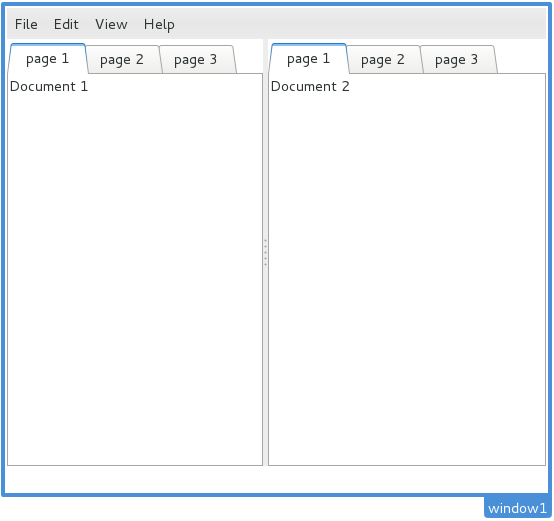
\includegraphics[scale=0.40]{./images/tab-groups-proto-1}
    \caption{Tab groups prototype 1}\label{fig:TabGroupsProto1}
  \end{minipage}
  \hspace{0.5cm}
  \begin{minipage}[b]{0.5\linewidth}
    \centering
    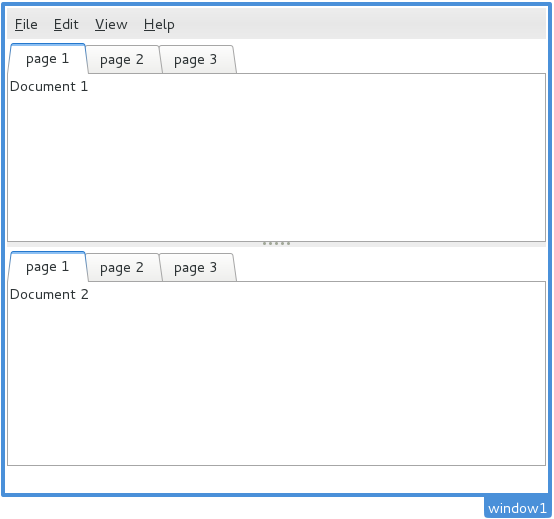
\includegraphics[scale=0.40]{./images/tab-groups-proto-2}
    \caption{Tab groups prototype 2}\label{fig:TabGroupsProto2}
  \end{minipage}
\end{figure}

\subsection{User interface}

To interact with tab groups, it was decided to provide three new menu items in the \emph{Documents} menu.
\begin{itemize}
  \item \textbf{New Tab Group:} It creates a tab group in the right of the focused one, and it adds a new tab to it.
  \item \textbf{Previous Tab Group:} Moves the focus to the previous (left) tab group.
  \item \textbf{Next Tab Group:} Moves the focus to the next (right) tab group.
\end{itemize}

\newpage
\subsection{Class diagram modification}

\addfigure[scale=0.45]{./images/tab-groups-diagram}{Tab groups diagram}{fig:TabGroupDiagram}

As it can be visualized in the figure \ref{fig:TabGroupDiagram} a new class has been introduced, \emph{GeditMultiNotebook}. This class will take care of create and remove GeditNotebooks, proxying the signals emittion for page-added, page-removed and switch-page and it will be kept as an implementation detail where the user will not have direct access to its API.

\newpage
\subsection{GeditMultiNotebook}

This class works as a proxy to \emph{GeditNotebook}, most of the API and signals are the same, here will be explained the different methods and signals.

\subsubsection{Signals}

\begin{table}[H]
  \begin{center}
    \begin{tabularx}{\textwidth}{|l|X|}
      \firsthline
      \textbf{Signal name:} & \textbf{Explanation:} \\
      \hline
      \textit{notebook\_added} & emitted when a new notebook has been added. \\
      \hline
      \textit{notebook\_removed} & emitted when a notebook is removed. \\
      \hline
      \textit{tab\_added} & proxy signal for page\_added from GtkNotebook. \\
      \hline
      \textit{tab\_removed} & proxy signal for page\_removed from GtkNotebook. \\
      \hline
      \textit{switch\_tab} & proxy signal for switch\_page from GtkNotebook. \\
      \hline
      \textit{tab\_close\_request} & proxy signal for tab\_close\_request from GeditNotebook. \\
      \hline
      \textit{page\_reordered} & proxy signal for page\_reordered from GtkNotebook. \\
      \hline
      \textit{show\_popup\_menu} & emitted when the right button of the mouse is clicked in the notebook. \\
      \lasthline
    \end{tabularx}
    \caption{Tab groups signals explanation}
  \end{center}
\end{table}

\begin{table}[H]
  \begin{center}
    \begin{tabularx}{\textwidth}{|l|X|}
      \firsthline
      \textbf{Method name:} & \textbf{Explanation:} \\
      \hline
      \textit{get\_active\_notebook} & Gets the active notebook, in order to know which one is the active, a track on the focused widget has to be taken. For this can be listened to the signal \emph{set-focus-child}. \\
      \hline
      \textit{get\_n\_notebooks} & Gets the number of notebooks, at least there will be one. \\
      \hline
      \textit{get\_nth\_notebook} & Gets the n notebook of the list. \\
      \hline
      \textit{get\_notebook\_num} & Given a notebook get the number in the list. \\
      \hline
      \textit{get\_n\_tabs} & Returns the number of tabs in all the notebooks. \\
      \hline
      \textit{get\_page\_num} & Finds the index of the page which contains the given tab. \\
      \hline
      \textit{get\_active\_tab} & Gets the active tab. \\
      \hline
      \textit{set\_active\_tab} & Sets the active tab. \\
      \textit{set\_current\_page} & Sets the active tab in relation to the total pages. \\
      \hline
      \textit{get\_all\_tabs} & Gets all the tabs. \\
      \hline
      \textit{close\_tabs} & Closes a list of tabs. \\
      \hline
      \textit{close\_all\_tabs} & Closes all tabs. \\
      \lasthline
    \end{tabularx}
  \end{center}
\end{table}

\newpage
\begin{table}[H]
  \begin{center}
    \begin{tabularx}{\textwidth}{|l|X|}
      \firsthline
      \textit{add\_new\_notebook} & Adds a new notebook. \\
      \hline
      \textit{remove\_active\_notebook} & Removes the active notebook. \\
      \hline
      \textit{previous\_notebook} & Focuses the previous notebook. \\
      \hline
      \textit{next\_notebook} & Focuses the next notebook. \\
      \lasthline
    \end{tabularx}
    \caption{Tab groups methods explanation}
  \end{center}
\end{table}

GTK+ provides a widget called \emph{GtkHPaned}, which is a container with two children arranged horizontally. An intensive use of this widget is needed in order to arrange the tab groups side by side.

The next pseudocode shows how it must be implemented:
\begin{lstlisting}[style=GObject]

void
add_notebook(new_notebook, main_container)
{
	if (main_container)
		main_container(new_notebook)
	else {
		paned = new_paned()
		parent = active_notebook.get_parent()
		parent.remove(active_notebook)
		parent.add(paned)

		paned.add1(active_notebook)
		paned.add2(new_notebook)
	}
	/* keep track of it in a list */
	notebooks.append(new_notebook)

	emit(notebook-added)
}

void
remove_notebook (notebook)
{
	if (notebooks.next() != NULL)
	{
		warning("Removing main notebook is not possible)
		return
	}

	ref(notebook)
	notebook.destroy()

	next = notebooks.next()
	parent = notebook.parent()
	children = parent.get_children()
	if (!children.next())
	{
		warning("parent must be a GtkPaned")
		return
	}

	grandpa = parent.parent()
	parent.remove(children[0])
	parent.destroy()
	grandpa.add(children[0])
	emit (notebook-removed, notebook)
	unref(notebook)
	focus(next)
}

\end{lstlisting}

\newpage
\section{Implementation}

To implemented this, there was one thing depending directly on GeditNotebook. \emph{GeditDocumentsPanel} (see figure \ref{fig:GeditDocumentsPanel1}), which shows in the side panel the currently opened documents and allows to manage them. This feature was disabled in order to be able to start the implementation.

\addfigure[scale=0.60]{./images/gedit-documents-panel1}{Documents panel}{fig:GeditDocumentsPanel1}

\subsection{Bugs}

In the next links it can be checked the patches provided and the revisions by the other developers:

\noindent\url{https://bugzilla.gnome.org/show_bug.cgi?id=619608} \\
\noindent\url{https://bugzilla.gnome.org/show_bug.cgi?id=620502}

\newpage
\section{Tests}

\begin{table}[H]
  \begin{center}
    \begin{tabularx}{\textwidth}{|X|X|l|}
      \firsthline
      \textbf{Test:} & \textbf{Expected result:} & \textbf{Test passed?} \\
      \hline
      Click on new tab group & Adds a new tab group, and a new document on it & Yes \\
      \hline
      Close last tab & Closes the latest tab and removes the tab group & Yes \\
      \hline
      Click on previous tab group & Moves to the previous tab group & Yes \\
      \hline
      Click on next tab group & Moves to the previous tab group & Yes \\
      \hline
      Drag and drop between tabs & Allows to move a tab between tab groups & Yes \\
      \hline
      Change tab group & Reflects the active tab group in the documents menu, setting the shortcuts to the active one & Yes \\
      \lasthline
    \end{tabularx}
    \caption{Tests tab groups}
  \end{center}
\end{table}

% mainfile:main.tex
% revised by dnolivieri

\chapter{Drag and Drop of Tabs}

%FIXME first draft

\section{Analysis and design}

As described in the previous chapter, a \emph{modification} in the drag and drop system had to be made. gedit's custom drag and drop was implemented a few years ago, when GtkNotebook did not have a way to do it by itself. This was implemented in GTK+ since the version 2.12, but it had a problem holding the port of gedit, it did not permit drag a tab out of the window to create a new window with this tab attached to it. This changed with the introduction of the \emph{create-window} signal from GtkNotebook, which is emitted when a tab is dropped out of the main window.

To implement this the next things are needed:
\begin{itemize}
  \item Remove all the legacy code from the custom implementation.
  \item Proxy the \emph{create-window} signal from GtkNotebook to GeditMultiNotebook.
  \item Listen to this signal in \emph{gedit-window}.
  \item When the signal is emitted,  clone the window and return to the signal the new active notebook, so GTK+ can know to which GtkNotebook add the dragged tab.
\end{itemize}

Note that with this implementation,  we will still have one regression: we will not be able to drop a tab in the view. From the documentation: If you want a widget to interact with a notebook through DnD (i.e.: accept dragged tabs from it),  it must be set as a drop destination and accept the target "GTK\_NOTEBOOK\_TAB". The notebook will fill the selection with a GtkWidget** pointing to the child widget that corresponds to the dropped tab.

\section{Implementation}

Once the analysis and design had been done, the implementation was straightforward.   It was a matter of:
\begin{itemize}
  \item \emph{setting a group name}: Notebooks with the same name will be able to exchange tabs via drag and drop. A notebook with a NULL group name will not be able to exchange tabs with any other notebook.
  \item \emph{proxy} the signal and \emph{listen} to it.
  \item \emph{add "GTK\_NOTEBOOK\_TAB"} to the list of DnD targets of the view and implement the receiving for it. Code shown below.
  \item extra care had to be  given  when implementing this to have the signals emitted in the \emph{right order}.
\end{itemize}

\begin{lstlisting}[style=GObject]

/* This goes in the constructor of the notebook class */
#define GEDIT_NOTEBOOK_GROUP_NAME "GeditNotebookGroup"
gtk_notebook_set_group_name (GTK_NOTEBOOK (notebook),
                             GEDIT_NOTEBOOK_GROUP_NAME);

/* Snippet of code for the received part of code needed for the view */
else if (info == TARGET_TAB)
{
	GtkWidget *notebook;
	GtkWidget *new_notebook;
	GtkWidget *page;

	notebook = gtk_drag_get_source_widget (context);

	if (!GTK_IS_WIDGET (notebook))
	{
		return;
	}

	page = *(GtkWidget **) gtk_selection_data_get_data (selection_data);
	g_return_if_fail (page != NULL);

	/* We need to iterate and get the notebook of the target
	   view because we can have several notebooks per window */
	new_notebook = get_notebook_from_view (widget);

	if (notebook != new_notebook)
	{
		gedit_notebook_move_tab (GEDIT_NOTEBOOK (notebook),
			                 GEDIT_NOTEBOOK (new_notebook),
			                 GEDIT_TAB (page),
			                 0);
	}

	gtk_drag_finish (context, TRUE, TRUE, timestamp);
}

\end{lstlisting}

\subsection{Bug}

In the next link, the patches provided and the revisions by the other developers  can be checked: 

\noindent\url{https://bugzilla.gnome.org/show_bug.cgi?id=456959}

\newpage
\section{Tests}

\begin{table}[H]
  \begin{center}
    \begin{tabularx}{\textwidth}{|X|X|l|}
      \firsthline
      \textbf{Test:} & \textbf{Expected result:} & \textbf{Test passed?} \\
      \hline
      Reorganize tabs & The tab was kept in the desired position & Yes \\
      \hline
      Drop a tab out of the window & A new window was created, the tab was attached to it and detached from the source window & Yes \\
      \hline
      Drop a tab in other window view & The tab is detached from the source window and attached to the target window & Yes \\
      \hline
      Create one tab group and drop a tab on it & The tab is detached from the source tab group and attached to the target one & Yes \\
      \hline
      Create one tab group and drop the last tab on another tab group & The tab is detached from the source tab group, the source tab group is removed and the tab is attached in the target tab group & Yes \\
      \lasthline
    \end{tabularx}
    \caption{Tests for new Drag and Drop system}
  \end{center}
\end{table}

% mainfile:main.tex

\chapter{libpeas}\label{chap:libpeas}

A decision was made several years ago to try and convert the plugin system used in gedit into an standalone library. The main reason for this, was that several applications were copying the gedit plugin system and then making small modifications on it to adapt it as they preferred.  The main reason for not making this fix in prior versions was based upon maintaining the ABI stability for the production level code with a large user base.
As explained in the chapter \ref{chap:GFile}, the version update to \GNOME 3.0 provided an opportunity to effect this risky change.

With the help of the rest of the \emph{gedit team}, Steve Fr\'ecinaux was the one that took care of creating this library. Even if I am not the one who created this code,  I provided significant help both in the design and to port gedit (together with other applications), thereby 
indicating problems and providing some patches. This chapter provides an overview of the whole port, the changes in the design,  
and how it changed the implementation of plugins, pointing out examples and the advantages of the new design.

Note that one of the design decisions when libpeas was implemented was to make it gobject-introspection based (see \ref{sec:GObjectIntrospection}). This was one of the main problems, the port to use this library was not straightforward.

\section{Analysis and Design}

\subsection{Old Plugin system}\label{sec:OldPluginSystem}

\addfigure{./images/libpeas1}{Old Plugin system diagram}{fig:OldPluginSystemDiagram}

In Figure \ref{fig:OldPluginSystemDiagram}, the class diagram of the plugin system was checked before 
any work was done in the libpeas library. In order to better understand the next parts of this chapter, an overview of the 
main classes in this diagram is needed.

\subsubsection{GeditPluginsEngine}

This is the main class of the plugin engine. It takes care of loading and unloading a specific plugin, activate and deactivate the plugins for a specific window and to get the information for a specific plugin.

The GeditWindow has a direct link to this class by telling to it when it has to activate or deactivate a plugin. Also, it listens to the signals `activate\_plugin' and `deactivate\_plugin' (which should be called `load\_plugin' and `unload\_plugin') to actually activate them.

This class is a singleton so it can be accessed at any point by any class.

\newpage
\subsubsection{GeditPluginManager}

\addfigure[scale=0.5]{./images/gedit-plugins-dialog}{Gedit plugins dialog}{fig:GeditPluginsDialog}

In Figure \ref{fig:GeditPluginsDialog} the user interface is shown that  exposes gedit preferences dialog to be able 
to load or unload plugins. This widget calls to load or unload methods from GeditPluginsEngine. This later will emit 
the related signal listened by the window as spotted before.

\subsubsection{GeditPlugin}

This is the class implemented by each plugin. It has the methods that each plugin has to implement.

\subsubsection{Other classes}

The rest of the classes are mainly an implementation detail which are the ones in charge of loading a specific type of plugin, i.e Python vs C plugins.

\newpage
\subsection{First design with libpeas}

\addfigure[scale=0.5]{./images/libpeas2}{First design using libpeas}{fig:FirstDesignUsingLibpeas}

In the design given in Figure \ref{fig:FirstDesignUsingLibpeas}, the design is similar to the previous case. Libpeas 
takes the classes from \ref{sec:OldPluginSystem} and exposes the public ones for the user. We can see that we 
still have a GeditPluginsEngine, the reason for this is explained below.

\subsubsection{GeditPluginsEngine}

This is a lightweight object inherited from PeasEngine. PeasEngine is the same as the previous GeditPluginsEngine, although it does not 
initialize the paths where to search the plugins, the name of the plugins etc. Here is where it takes part the new GeditPluginsEngine, 
it initializes the super class by setting the name of the application and the plugin paths.

\subsection{Second design with libpeas}

\addfigure[scale=0.45]{./images/libpeas3}{Design using extensions}{fig:DesignExtensions}

One of the most frustrating limitations of the gedit plugins engine was that it only allows 
the extention of a single class, called GeditPlugin. With libpeas, this limitation vanishes, 
and the application writer is now able to provide a set of interfaces the plugin writer will be able to implement as the plugin requires.

In this design, we make use of the extension points. As we can see there are three extension points:
\begin{itemize}
  \item \textbf{GeditAppActivatable}: They are extensions that need to be instantiated per application instance. They will be accessible by all the windows. This is interesting if we want to read some specific data and create a singleton for it.
  \item \textbf{GeditWindowActivatable}: Extensions which interact directly with a window. For example the need to add a side pane or a bottom pane, menu items etc.
  \item \textbf{GeditViewActivatable}: Extensions which need either add new things to the document view, or to manage the document buffer to add new edition features.
\end{itemize}

For this, libpeas exposes a new class PeasExtensionSet. A PeasExtensionSet is a class that helps to manage all the specific extensions. As one plugin can adds one or more extensions, for example the window will have to deal with all the WindowActivatable extensions created by all the plugins. PeasExtensionSet ensures the life of each of them and allows the container class (GeditWindow) to send activations, deactivations or other calls needed to this extensions.

Apart from this new feature, the design is kept the same. The only problem is that it will produce a lot of work 
for porting the old plugins to this new design. In the next sections is shown an overview of how it had to be dealt 
with this in order to port the old plugins.

\newpage
\section{Old Plugin implementation}

Here a snippet is shown that indicates how the previous plugin looked:

\subsection{Minimalist plugin}

\begin{lstlisting}[style=python]

import gedit

class ExamplePyPlugin(gedit.Plugin):
    def activate(self, window):
        pass

    def deactivate(self, window):
        pass

    def update_ui(self, window):
        pass

\end{lstlisting}

As we can be seen in this example, each plugin must implement three methods:
\begin{enumerate}
  \item \textbf{activate:} called when the plugin is activated. This is usually used for the initialization of the plugin itself.
  \item \textbf{deactivate:} called when the plugin is deactivated. Used to dispose the plugin.
  \item \textbf{update\_ui:} called when a change in user interface of the window has been introduced. i.e when a tab in the window has been switched.
\end{enumerate}

\subsection{Window controller}\label{sec:WindowController}

As was explained in chapter \ref{chap:InitialAnalysis}, gedit is a \emph{single instance application}. This means that for each instance of the application we can have several windows. This is applied also to the plugins. One plugin instance will be created only once, and then the activate/deactivate/update\_ui methods will be called for each window.

This has forced us to introduce the \emph{window controller}, which is one class that takes care to control a specific window. The plugin instance will have a hash table that takes care of calling the right window controller instance method. This allows a simple way to implement plugins.

The main problem with this was that each plugin developer needed to know internal details of gedit in order to create a plugin correctly. In the example below, it can be shown how it was dealed with this before.

\begin{lstlisting}[style=python]

import gedit

class ExamplePyWindowHelper:
    def __init__(self, plugin, window):
        print "Plugin created for", window
        self._window = window
        self._plugin = plugin

    def deactivate(self):
        print "Plugin stopped for", self._window
        self._window = None
        self._plugin = None

    def update_ui(self):
        # Called whenever the window has been updated (active tab
        # changed, etc.)
        print "Plugin update for", self._window

class ExamplePyPlugin(gedit.Plugin):
    def __init__(self):
        gedit.Plugin.__init__(self)
        self._instances = {}

    def activate(self, window):
        self._instances[window] = ExamplePyWindowHelper(self, window)

    def deactivate(self, window):
        self._instances[window].deactivate()
        del self._instances[window]

    def update_ui(self, window):
        self._instances[window].update_ui()

\end{lstlisting}

\section{New plugin implementation}

A plugin will be able to have one or more extensions. Each extension is derived from GObject.Object and must implement one of the interfaces that gedit provides for the extension points.

\begin{lstlisting}[style=python]

from gi.repository import GObject, Gedit

class ExamplePyWindowActivatable:
    __gtype_name__ = "ExamplePyWindowActivatable"

    window = GObject.property(type=Gedit.Window)

    def __init__(self):
        GObject.Object.__init__(self)

    def do_activate(self):
        print "Plugin created for", self.window

    def do_deactivate(self):
        print "Plugin stopped for", self.window

    def do_update_state(self):
        # Called whenever the window has been updated (active tab
        # changed, etc.)
        print "Plugin update for", self.window

\end{lstlisting}

This example provides the same as the one provided in the section \ref{sec:WindowController}. As we can see, it is a lot easier to implement and it needs a smaller learning curve. For each window, a new extension point is created so the class ExamplePyWindowActivatable will be instantiated for each of them.

\section{Tests}

Unfortunately, to test this, we had to check all the functionalities. The main problem with this was that we had to port also the python plugin to use gobject-introspection. This meant that the methods did not take the same amount of arguments, and thus we needed to test all the code base and all the functionalities, one by one.


% mainfile:main.tex

\chapter{New search system}

\section{Analysis and Design}

\addfigure[scale=0.75]{./images/gedit-old-find}{Old search dialog}{fig:OldFind}

As can be seen in Figure \ref{fig:OldFind}, gedit's search dialog has not evolved over the past years. This way of presenting 
a search dialog to the user poses a signicant problem: it obscures the text you are searching for. In the past few years, a few popular applications 
such as Firefox or Chrome have invented several ideas, which are the methods presently employed by most software applications 
for searching within the documents.

\newpage
\subsection{Firefox vs Chrome}

In figure \ref{fig:FirefoxSearch}, the method used by Firefox is shown that presents a search prompt to the user. This method has a few problems.
\begin{itemize}
  \item Some studies have demonstrated that presenting visual elements to the user in the bottom of a screen are less discoverable 
   than elements in the top-left of the screen.
  \item It resizes the web browser viewer to present the search widget. This also has an advantage, it will not obscure any part of the document.
  \item It takes a big part of horizontal space.
\end{itemize}

\addfigure[scale=0.5]{./images/firefox-search}{Firefox search}{fig:FirefoxSearch}

As shown in Figure \ref{fig:ChromeSearch}, Chrome utilizes an idea based upon the Firefox search, yet tries to fix some of the problems. Nonetheless, this solution is still not perfect.
\begin{itemize}
  \item It shows the pop up in the top-right, which is not the top-left as the studies demonstrated. Although, this is still better than in the bottom of the screen.
  \item It obscures part of the document.
\end{itemize}

\addfigure[scale=0.5]{./images/chrome-search}{Chrome search}{fig:ChromeSearch}

In the analysis of the currently used search systems, we can see that there is no perfect system to manage a search by the user. In gedit, after some discussion, we decided that the best option for gedit would be one similar to Chrome' search widget approach.  The principal reason is that we believe people write more vertically than horizontally.  Thus, poping out a widget on the top-right of the screen should not pose a significant problme to the user. Also, this solution seemed to be the lesst problematic search method based upon our understanding.

\subsection{Current design}

Figure \ref{fig:OldClassDiagram} shows the appearance  of the current design before introducing anything new, in order to see how 
things will evolve.

***** Not sure what you mean **** clean this up..

\addfigure[width=\textwidth]{./images/search-system-old}{Old class diagram}{fig:OldClassDiagram}

\subsection{New design}

In Figure \ref{fig:SearchClassDiagram}, the new design is shown in order to implement the new search pop up. The main problem is that we do not have a container which will allows us to place a widget in a fixed position having a main widget below it. The only widget that allows for fixed positions in GTK+ is \emph{GtkFixed}.   The problem with this widget is that it does not allow a main widget design. Here is where we need to get the requisites for this widget:

\subsubsection{GeditOverlay}

GeditOverlay is a container which inherits from GtkContainer as any other implemented in the GTK+ toolkit. This container will need:
\begin{itemize}
  \item A main widget, which will allocate the whole space that can count with.
  \item A way to add a widget overlaying the main widget in fixed positions. For this we can use the vertical and horizontal alignments provided by GtkWidget.
\begin{lstlisting}[style=GObject]
typedef enum
{
  GTK_ALIGN_FILL,
  GTK_ALIGN_START,
  GTK_ALIGN_END,
  GTK_ALIGN_CENTER
} GtkAlign;
\end{lstlisting}
  \item A way to set an offset in case we do not want the added widget in the edge of the main widget. I.e like in the figure \ref{fig:ChromeSearch} where there is an extra space in the right.
  \item A way to animate a specific widget. See \ref{sec:Theatrics} for an explanation about this.
\end{itemize}

This widget does not add any specific API apart from gedit\_overlay\_add.

\begin{lstlisting}[style=GObject]
void	 gedit_overlay_add (GeditOverlay             *overlay,
			    GtkWidget                *widget,
			    GeditOverlayChildPosition position,
			    guint                     offset);
\end{lstlisting}

\subsubsection{GeditOverlayChild}

This widget is needed by GeditOverlay to wrap widgets added to it. The reason for this is that all widgets added in GeditOverlay need to be windowed and widgets like GtkEntry or GtkLabel are not windowed. So the main target for GeditOverlayChild is to create a window and set the added widget to this window.

\subsubsection{GeditFloatingSlider}

Inherits from GeditOverlayChild. This widget will be wrapped as a GeditTheatricsActor and in each iteration set its window size to the percent of the animation. In this way we will have a slide in or out effect depending on the moment of the animation.

\subsubsection{GeditRoundedFrame}

GTK+ GtkFrame does not provide any way to draw a rounded frame. This widget is more like a stylish way for making prettier the search widget and does not provides any specific capabilities except the stylistic one.

\subsubsection{GeditViewFrame}

GeditViewFrame is a delegate widget in order to remove complexity from GeditTab. This widget will take care of creating the Overlay, the View and the Document and add them correctly.

Apart from that, it will also take care of managing the search widget, setting when it must do a specific animation and provide API to invoke it from the GeditWindow's menu.

The API provided by this widget is:

\begin{table}[H]
  \begin{center}
    \begin{tabularx}{\textwidth}{|X|X|}
      \firsthline
      \textbf{Method name:} & \textbf{Explanation:} \\
      \hline
      get\_document & Gets the GeditDocument. This is an utility method to not have to get the view and get the buffer from the view. \\
      \hline
      get\_view & Gets the GeditView. \\
      \hline
      popup\_search & Shows the search pop up. \\
      \hline
      clear\_search & Removes any highlighted occurrences in the text. \\
      \lasthline
    \end{tabularx}
    \caption{GeditViewFrame methods explanation}
  \end{center}
\end{table}

\subsubsection{GeditSearchWidget}

This widget is a simple box container, since it adds the entry and the buttons to go to the next occurrence or to the previous one. It will listen to the changes on the entry text and search in the document as appropriate. It will also launch a dropdown menu to configure the type of search that it wants to be set.

\newpage
\addfigure[scale=0.45]{./images/search-system}{Search class diagram}{fig:SearchClassDiagram}

\newpage
\subsection{Theatrics}\label{sec:Theatrics}

With the design shown in Figure \ref{fig:SearchClassDiagram}, the class is almost complete. The principal problem that remains is that we do not have a way to animate the pop up. GTK+ does not provide any way for doing such animations and the only way is to create it by using a timeout and make the animation in each iteration. In Figure \ref{fig:Theatrics}, the design for a custom framework to help to achieve this is shown.

\addfigure[scale=0.40]{./images/theatrics}{Theatrics}{fig:Theatrics}

\subsubsection{GeditTheatricsActor}

Wraps a specific object to animate it. Below are shown the methods of this class.

\begin{table}[H]
  \begin{center}
    \begin{tabularx}{\textwidth}{|X|X|}
      \firsthline
      \textbf{Method name:} & \textbf{Explanation:} \\
      \hline
      reset & Resets the actor and sets the new duration. \\
      \hline
      get\_target & Gets the specific object that it is animating. \\
      \hline
      get\_expired & Gets if the animation has expired. \\
      \hline
      get\_can\_expire & Gets if the animation can expire. \\
      \hline
      set\_can\_expire & Sets if the animation can expire, if it can not expire the animation behaves like a loop. \\
      \hline
      get\_duration & Gets the duration of the animation. \\
      \hline
      get\_start\_time & Gets the initial time of the animation. \\
      \hline
      get\_frames & Gets the number of frames. \\
      \hline
      get\_frames\_per\_second & Gets the number of frame in a second. \\
      \hline
      get\_percent & Gets the percent of the already done animation. \\
      \lasthline
    \end{tabularx}
    \caption{Actor methods explanation}
  \end{center}
\end{table}

\newpage
\subsubsection{GeditTheatricsStage}

It is the class that manages the actors. This class stores them, creates the timeouts for the animations and emits a signal \emph{actor-step} indicating the steps of the animation from each actor.

\begin{table}[H]
  \begin{center}
    \begin{tabularx}{\textwidth}{|X|X|}
      \firsthline
      \textbf{Method name:} & \textbf{Explanation:} \\
      \hline
      add & Adds an object to be animated and it wraps it into an actor. \\
      \hline
      add\_with\_duration & Utility method that makes the same as add but also establishing a specific duration for the actor. \\
      \hline
      remove & Removes the object from the stage to not animate it anymore. \\
      \hline
      set\_playing & Sets whether the animation is running or not. \\
      \hline
      get\_playing & Gets whether the animation is running or not. \\
      \lasthline
    \end{tabularx}
    \caption{Stage methods explanation}
  \end{center}
\end{table}

\section{Implementation}

To implement this feature, a new branch was used to make it easy to develop it and test. When it was ready it was squashed into a single patch and attached to the bug report below.

\subsection{Bug}

\url{http://bugzilla.gnome.org/show_bug.cgi?id=419805}

\newpage
\section{Tests}

\begin{table}[H]
  \begin{center}
    \begin{tabularx}{\textwidth}{|X|X|l|}
      \firsthline
      \textbf{Test:} & \textbf{Expected result:} & \textbf{Test passed?} \\
      \hline
      Press \emph{Control + F} or \emph{Search $\to$ Find} & The search pop up appears, sliding out with an animation & Yes \\
      \hline
      Write some text that appears in the document & The first occurrence is selected and the others are highlighted & Yes \\
      \hline
      Write some text that do NOT appear in the document & The search entry color changes to an error color and no text is selected or highlighted & Yes \\
      \hline
      With several occurrences highlighted, press the Up button, or the Up arrow key from the keyboard & The previous occurrence should be selected & Yes \\
      \hline
      With several occurrences highlighted, press the Down button, or the Down arrow key from the keyboard & The next occurrence should be selected & Yes \\
      \hline
      Pressing \emph{ESC} with the search pop up opened & The search dialog should slide out and go back to the position before it was opened & Yes \\
      \hline
      Pressing \emph{Enter} with the search pop up opened & The search dialog should slide out and keep the cursor in the selected occurrence & Yes \\
      \hline
      Configure the dropdown menu & The changes are set correctly and the text is searched in relation to those changes & Yes \\
      \lasthline
    \end{tabularx}
    \caption{Tests for new search system}
  \end{center}
\end{table}

% mainfile:main.tex

\chapter{Invalid characters}

\section{Analysis and Design}

In the version gedit 2.30 we introduced a new way for opening and saving files by using input and output streams. An input stream allows us to read an stream from a specific source and attach to it GFilterInputStreams to make operations on it while we are reading the specific stream. An output stream allows us to write data in one source and attach GFilterOutputStreams to make operations in the written data. In the figures \ref{fig:InputStreams} and \ref{fig:OutputStreams}, we can check the diagrams of how gedit deals right now with this two situations.

\addfigure[scale=0.5]{./images/input-streams}{gedit input streams flow diagram}{fig:InputStreams}

\addfigure[scale=0.5]{./images/output-streams}{gedit output streams flow diagram}{fig:OutputStreams}

In this chapter we are going to focus on the input streams, as we want to escape the invalid characters and show them to the user. Here it will be explained what are the input streams used for.

\subsection*{GFileInputStream}

This is the stream that takes care of reading a buffer from a specific file asynchronously and pass the data to the next level in each iteration.

\subsection*{GConverterInputStream}

A GConverterInputStream is a GFilterInputStream which allows to set one type of GConverter object. In this case we have two different ones. The first one allows to open compressed files. For example a gzip file is opened with gedit, this data is read by GFileInputStream and passed to this FilterStream which deal with the decompression using the GZlibDecompress object.

Once the file is decompressed, in case the file is a compressed file, it is passed to another GConverterInputStream. This FilterStream deals with the encodings. GTK+ only manages UTF-8 encoding text so need to make the conversion to it before adding anything to the text buffer.

\subsection*{GeditDocumentOutputStream}

This is not an input stream, but an output stream. The reason for this is that it takes care of writing the buffer that came from the upper levels to the GtkTextBuffer. This output stream also deals with detecting whether or not the text provided is an UTF-8 valid text or not and finally write it in the GeditDocument object.

\section{Implementation}

\subsection{Bug}

\noindent\url{https://bugzilla.gnome.org/show_bug.cgi?id=502947}

\section{Tests}

To test this implementation, it was used a set of unit tests. This is a very low level implementation and one of the most important part of gedit, as we have to ensure that the data will not get lost and will be valid.

\begin{lstlisting}[style=GObject]
static void
test_consecutive_write (const gchar *inbuf,
			const gchar *outbuf,
			gsize write_chunk_len,
			GeditDocumentNewlineType newline_type)
{
	GeditDocument *doc;
	GOutputStream *out;
	gsize len;
	gssize n, w;
	GError *err = NULL;
	gchar *b;
	GeditDocumentNewlineType type;
	GSList *encodings = NULL;

	doc = gedit_document_new ();
	encodings = g_slist_prepend (encodings, (gpointer)gedit_encoding_get_utf8 ());
	out = gedit_document_output_stream_new (doc, encodings);

	n = 0;

	do
	{
		len = MIN (write_chunk_len, strlen (inbuf + n));
		w = g_output_stream_write (out, inbuf + n, len, NULL, &err);
		g_assert_cmpint (w, >=, 0);
		g_assert_no_error (err);

		n += w;
	} while (w != 0);

	g_output_stream_flush (out, NULL, &err);

	g_assert_no_error (err);

	type = gedit_document_output_stream_detect_newline_type (GEDIT_DOCUMENT_OUTPUT_STREAM (out));
	g_assert (type == newline_type);

	g_output_stream_close (out, NULL, &err);
	g_assert_no_error (err);

	g_object_get (G_OBJECT (doc), "text", &b, NULL);

	g_assert_cmpstr (outbuf, ==, b);
	g_free (b);

	g_assert (gtk_text_buffer_get_modified (GTK_TEXT_BUFFER (doc)) == FALSE);

	g_object_unref (doc);
	g_object_unref (out);
}

static void
test_invalid_utf8 ()
{
	test_consecutive_write ("foobar\n\xef\xbf\xbe", "foobar\n\\EF\\BF\\BE", 10,
	                        GEDIT_DOCUMENT_NEWLINE_TYPE_LF);
	test_consecutive_write ("foobar\n\xef\xbf\xbezzzzzz\n", "foobar\n\\EF\\BF\\BEzzzzzz", 10,
	                        GEDIT_DOCUMENT_NEWLINE_TYPE_LF);
	test_consecutive_write ("\xef\xbf\xbezzzzzz\n", "\\EF\\BF\\BEzzzzzz", 10,
	                        GEDIT_DOCUMENT_NEWLINE_TYPE_LF);
}
\end{lstlisting}

In this tests, we check that introducing some text with invalid characters at the end, middle and beginning of a string, we get them escaped getting the expected result and without getting any error in the operation.

\chapter{GTK+ 3.0}

\part{User manual}
% mainfile:main.tex

\chapter{Tab groups}

One of the main points for any \GNOME application is to provide an easy to use user interface. To manage the tab groups three menu items were provided, as shown in the figure \ref{fig:DocumentsMenu}. Below you can find a explanation of each menu item in detail:
\begin{itemize}
  \item \textbf{New Tab Group:} It creates a new tab group in the right side of the active document, with a new document on it.
  \item \textbf{Previous Tab Group:} Moves the focus to the tab group on the left. If there is no tab group on the left it moves the focus to the last tab group.
  \item \textbf{Next Tab Group:} Moves the focus to the tab group on the right. If there is no tab group on the right it moves the focus to the first tab group.
\end{itemize}

\addfigure[scale=0.50]{./images/documents-menu}{Documents menu}{fig:DocumentsMenu}

In the figure \ref{fig:UserTabGroups}, it can be visualized an example of how it would look a gedit window with two tab groups and several docuements opened on each of them.

\addfigure{./images/user-tag-groups}{Tag groups}{fig:UserTabGroups}

% mainfile:main.tex
% revised by dnolivieri
\chapter{Search system}

\section{Show the search pop up}

In Figure \ref{fig:SearchPopup}, the appearance of the new search pop up is shown. In order to launch the search search pop up, the user 
can do it in two possible ways:  Pressing \emph{Control + F} or going to the menu \emph{Search $\to$ Find}.

\addfigure[scale=1.0]{./images/search1}{Search popup}{fig:SearchPopup}

\section{Configure the search pop up}

As can be seen in Figure  \ref{fig:SearchPopupMenu}, when a search for some text is desired, the user can select 
several options to restrict the search. By default,  the less restrictive search will be provided. In order to  launch the drop 
down menu,  it should be clicked in the lens icon, either with the left or right button of the mouse. The 
following is a description of each item in the dropdown menu:
\begin{itemize}
  \item \textbf{Match Case:} It will make the search case sensitive.
  \item \textbf{Match Entire Word Only:} It will only match whole words.
  \item \textbf{Wrap Around:} This option will make the search engine restart from the beginning once the end of the document is reached.
\end{itemize}

\addfigure[scale=1.0]{./images/search2}{Search pop up menu}{fig:SearchPopupMenu}

\section{Error reporting}

With this new search, an interactive search it is done. When an occurrence is not found in the document,  the way that it is reported 
to the user is by turning the search entry into red as shown in the figure \ref{fig:SearchPopupError}.

\addfigure[scale=1.0]{./images/search3}{Search pop up error}{fig:SearchPopupError}

\newpage
\section{Match visualizing}

When doing an interactive search,  there are two visual reports. The active match and the matches around the document. 
In the casse of the active match,  it is the selected text found where the cursor is placed. The matches found 
in the document are visualized 
in a different color depending on the theme and it shows all the occurrences for the searched text in the document.

\addfigure[scale=1.0]{./images/search4}{Search pop up interactive search}{fig:SearchPopupInteractive}

\section{Interaction}

To interact with the search pop up, there are several ways, as described below:
\begin{itemize}
  \item \textbf{Search for text:} It is a matter of entering some specific text in the entry text.
  \item \textbf{Select the entry text:} Apart from the usual methods, it can be also selected by pressing again \emph{Control + F}.
  \item \textbf{Move between occurrences:} To do this, we can do it by clicking in the arrow buttons, by pressing the arrow keys of the keyboard or by pressing \emph{Control} and scrolling with the mouse.
  \item \textbf{Close the pop up:} There are two ways to do it:
    \begin{itemize}
      \item \textit{Pressing ESC:} By pressing this key, the pop up is closed and the cursor is returned to the place before the search was done.
      \item \textit{Pressing Enter:} By pressing this key, the pop up is also closed but the cursor is kept on the selected occurrence.
    \end{itemize}
\end{itemize}


\appendix
% mainfile:main.tex

\chapter{Work flow using Git}

\emph{Git} is a very powerful tool, used by many important projects like the \emph{Linux kernel} and is the chosen one for the \GNOME desktop. The fact that it is so powerful it does not mean that it is very easy to use. Here it will be explained the main steps in order to have an overview of the main work flow.

Before explaining the main steps, it must be known that git manages everything with branches. The main branch, usually used for the development copy of the program is called: \emph{master}.

\section*{Get a copy of the software}

To make this it will be used the `clone' command:

\noindent\graybox{git clone git://git.gnome.org/gedit}

\section*{Committing a change}

In git it is a bit different than svn, it is splitted in two steps:

\noindent\graybox{git commit -a}

This command will make the change in the local branch, creating the specific commit. See also that we specify the `-a' argument so all changes in the branch are committed. If we want to stage specific changes we can use the command:

\noindent\graybox{git add file}

\noindent\graybox{git push origin branch\_name}

This other command will put the previous commit or commits in the remote branch.

\section*{Update the working copy}

\noindent\graybox{git pull --rebase}

See that here it is important to pass `--rebase', as if you have any commit in this specific branch before updating, you will want that commit to be in the top of the updated branch.

\section*{Wipe out previous changes}

\noindent\graybox{git checkout -f}

With this command will remove all the changes made in the current branch.

\noindent\graybox{git reset}

The previous command removes the changes made in a branch, although git reset, allows the user to drop out the specific commits you don't want.

\section*{Create a new branch}

\noindent\graybox{git checkout -b branch\_name}

It will create a new branch with the name `branch\_name'.

\section*{Switch between branches}

\noindent\graybox{git checkout branch\_name}

See that to be able to change the branch, it will be needed to have no changes on it.

\newpage
\section*{Merge branches}

\noindent\graybox{git merge branch\_name}

With this command a direct merge will be made, placing the commits in the places where it were made, and if there is any conflict a new commit will be made on the top fixing this conflicts.

\noindent\graybox{git rebase -i branch\_name}

It puts all the commits to be merged on top of the branch we want to put them. If there are conflicts, each commit with a conflict should be edited and fixed.

\section*{Remove a branch}

\noindent\graybox{git branch -D branch\_name}

This one will remove the local branch named with branch\_name.

\noindent\graybox{git push origin :branch\_name}

And this other will remove branch\_name in the remote server.

\section*{Creating a patch}

\noindent\graybox{git diff \textgreater~patch\_name}

It creates a file with patch\_name as name, with the local non committed changes.

\noindent\graybox{git format-patch origin}

It will create a patch for each new commit not pushed to the remote branch. The difference with the previous command is that this one conserve extra information, like the author of the commit.

\newpage
\section*{Apply a patch}

\noindent\graybox{git apply patch\_name}

It applies the patch on top of the local branch.

\noindent\graybox{git am patch\_name}

It applies the patch but it also creates the local commit with the extra information.

% mainfile:main.tex

\chapter{Making a release}

The first thing that you have to know when you are making a release, is whether the module is using pre-release version incrementing (i.e. bumping the version number just before release) or post-release version incrementing (which is preferred for libraries). gedit uses a pre-release version incrementing. This can be usually checked in the \emph{configure.in} or \emph{configure.ac} files. After this has been checked the next steps have to be followed:

\section*{Make sure you are up to date}

\noindent\graybox{git pull --rebase}

\section*{Make sure there are not local changes}

\noindent\graybox{git status}

\section*{Increment the version}

\noindent Modify configure.ac and modify the version.

\section*{Update the README file}

\noindent Usually you have to update the version number in all the occurrences in this document.

\section*{New entry in the NEWS file}

\noindent It should be read the ChangeLog and come up with a bullet point for each significant change and credit the person who did the work. Below it can be found an example and the command to show the ChangeLog:

\noindent\graybox{git log}

\begin{lstlisting}[style=plain]
============
gedit 2.91.6
============

New Features and Fixes
======================
- Fix encoding conversion (Ignacio Casal Quinteiro)
- Add invalid char support (Ignacio Casal Quinteiro, Paolo Borelli)
- More plugins ported to pygobject
- Misc bugfixes

New and updated translations
============================
- cs (Marek Cernocky)
- eo (Kristjan SCHMIDT)
- gl (Fran Dieguez)
- pa (A S Alam)
\end{lstlisting}

\section*{Recompile everything}

For this several commands have to executed:

\noindent\graybox{./autogen.sh --enable-gtk-doc}

\noindent\graybox{make}

\noindent\graybox{make install}

\newpage
\section*{Create the tarball\footnote{A tar file or compressed tar file is commonly referred to as a tarball.}}

The command below will create the tarball and automatically check that all files are added correctly to this compressed file, that everything compiles correctly and that all tests are passed.

\noindent\graybox{make distcheck}

Once distcheck finished, it should show something like this:

\begin{lstlisting}[style=plain]
==================================================
gedit-2.90.6.tar.xz is ready for distribution
==================================================
\end{lstlisting}

\section*{Commit}

\noindent\graybox{git commit -a}

\section*{Push the change}

\noindent\graybox{git push origin master}

If some change has been done in the repository before this step and the commit can not be pushed, it should go back to the first step and start over.

\section*{Tag the release}

\noindent\graybox{git tag -a 2.90.6}

See that the name of the tag will be the version of the release.

\section*{Push the tag}

\noindent\graybox{git push origin 2.90.6}

\newpage
\section*{Upload the tarball}

\GNOME provides a server where to upload the released tarball so other people can have access to them easily.

\noindent\graybox{scp gedit-2.90.6.tar.xz (user)@master.gnome.org:}

\section*{ssh into the server}

\noindent\graybox{ssh (user)@master.gnome.org}

\section*{Install the tarball in the server}

\noindent\graybox{ftpadmin install gedit-2.90.6.tar.xz}

Once it is installed you should get confirmation that it was correctly installed.

% mainfile:main.tex

\chapter{Google summer of code}

\emph{Google Summer of Code} is a global program that offers student developers stipends to write code for various open source software projects.\cite{website:soc}

Some of the features and bug fixes made in this project have been part of the \emph{Google summer of code 2010}. Here, an approximation will be shown to what is needed for applying for this Google \emph{internship} and what it has to be done in order to make it.

\addfigure[width=0.5\textwidth]{./images/gsoc}{GSoC 2010 Logo}{fig:GSoCLogo}

\newpage
\section{Proposing a good project}\label{sec:GoodProject}

There are several ways to propose a project for the Google summer of code. The main ones are:
\begin{itemize}
  \item Looking for a free software application that you really like, and propose something that you want to improve.
  \item Talk with the application maintainers and ask them for interesting projects that they would like to mentor. This is probably the most used way and the best way if you want to get your project \emph{accepted}.
\end{itemize}

Usually the accepted organizations by Google, they provide a wiki where they put some proposals for students, as an example, the one from \GNOME for 2010. See: \url{https://live.gnome.org/SummerOfCode2010}.

\section{Creating the application form}\label{ApplicationForm}

In the application form, it has to be described what you want to do, a schedule explaining what it will be done every week and something about you. Below it is shown the \emph{application form} I have used for my Google summer of code.

\subsection*{gedit improvements}

\subsubsection*{gedit split view}

Right now gedit does not have the ability to provide several views for the same document. I would like to change the internal design of gedit to provide this. The idea is that a document can be splitted horizontally or vertically depending on what the user prefers. For doing this some menu items will be provided.
Due to the current design of GtkTextView this is not an easy task as we need to load the document again every time we split it, and keep it sync.

\paragraph{Why is this important?}

It is important because it can allow you to see several parts of the same document at the same time, which is necessary when you are editing long files.

\subsubsection*{gedit tab groups}

Split view is a really good thing but does not provide a way to see different documents at the same time.

By tab groups we refer to the ability of grouping gedit tabs in different groups that can be viewed at the same time in a gedit window.
\begin{itemize}
  \item By default a gedit window has a single tab group (current behavior).
  \item The same document can NOT appear in different tab groups or different tabs.
\end{itemize}

\paragraph{Why is this important?}

It is important to compare different files side by side.

\subsubsection{gedit multi-views}

Apart from split view and tab groups, I'd like to add support (if time permits) for multi views. This means to add abstraction for the document and for the text viewer. In this way we could be able to open a binary file with its own viewer. Or watch a specific html file using webkit as the viewer.\footnote{\url{http://live.gnome.org/Gedit/Multiviews}}

\subsubsection{Timeline}

A proposed timeline (but highly flexible depending on the time needed):

\begin{itemize}
  \item Week 1 and 2: Provide a patch for being able to create tab groups.
  \item Week 3 and 4: See if we need to refactor code to maintain easier the tab groups and start with the split view patch.
  \item Week 5 and 6: Finish the split view patch and see if it need some refactor.
  \item Week 7 and 8: Start the work on the gedit view interface.
  \item Week 9 and 10: Finish the gedit view abstraction and see if worth start working the document abstraction or just bug fixing.
  \item Week 10 and 11: Finish the document abstraction if possible or make stability work.
\end{itemize}

\subsubsection{About me}

My name is Ignacio Casal Quinteiro, I'm 23 years old and I'm studying computer engineer at the Vigo University of Spain. I have been contributing to \GNOME for several years, from tasks like coordinating the Galician translation team to applications like gedit or gtranslator. I love free software and I love \GNOME, the community around it is just awesome, and I would really like to continue my contributions on making it better than it is right now. Even if I already contributed to \GNOME, this project would be a major rewrite of the gedit internals, and the amount of work involved is proportional to a good GSoC. Also making this GSoC would give me the opportunity to spend the summer working on \GNOME instead of another part time job.

\section{Reporting the work}\label{ReportingGSoC}

Depending on the organization, it will be different the way to report what it has been done every week. In the case of \GNOME it is mandatory to make three things:

\begin{itemize}
  \item Create a portfolio: this is a document in the wiki of \GNOME where it has to be explained what you project is about, where to find the code and the links to the documentation reported. For an example here is my portfolio: \url{https://live.gnome.org/SummerOfCode2010/IgnacioCasal_gedit}.
  \item Mail and blog post: every week it has to be sent a post and an email explaining what it has been done, what it will be done next week and if the timeline is under schedule. See one blog post \url{http://blogs.gnome.org/nacho/2010/07/25/gsoc-weekly-report-9/}.
\end{itemize}

% mainfile:main.tex
% revised by dnolivieri
\chapter{Python hackfest 2011}

%FIXME: ref to chapters
One of the problems encountered on the road to \GNOME 3.0 was that we bet on dynamic bindings, as explained in previous chapters, instead of keeping static ones. At the end of 2010, with just a couple of months before the stable release, we were still without an usable version of PyGObject working with introspection. This lead to propose a hackfest\footnote{A hackfest is a meeting in some place around the world, where developers discuss and fix problems related with a specific topic, i.e an application or library.}, where we could meet and focus on the main problems in order to get a stable release as soon as possible.

\section{Location, date}

Prague, CZ - Jan 17th-21st\\
Hackerspace Prague (brmlab)

\section{Goals}

\begin{itemize}
  \item Get a deeper understanding of what parts are important to GNOME Python and focus on getting those bits finished.
  \item Identify API in GTK+ that is unwrappable and get it fixed before the freeze.
  \item Work with developers to port their applications.
  \item Get PyGObject into a shippable, stable state.
  \item Figure out our post-GNOME 3.0 goals.
  \item Reduce invocation overhead.
  \item Move overrides to one or more separate modules.
  \item Figure out a way to have private overrides for applications (i.e gedit).
  \item Bugs to look at: \#561264, \#638915.
\end{itemize}

\section{Getting sponsor}

As explained on the web page \url{https://live.gnome.org/Travel}, the \GNOME Foundation supports the \GNOME project and one important way of doing that is sponsoring contributors to travel to \GNOME events like conferences and hackfests. The sponsored travel is meant to help those that would like to attend \GNOME related events but are unable to do so for financial reasons. All \GNOME contributors are always encouraged to apply.

The way to get sponsored, is to be a hacker of the \GNOME project and submit a document, specifying why the event it is needed,  the sponsorship, and the quantity of money needed. If the proposal is accepted, it is possible to attend to the event sponsored. The sponsor provides money for the travel and for the accommodation.

Apart from the \GNOME foundation, one important company in the free software world sponsored also this hackfest. Collabora\footnote{See: \url{http://www.collabora.com/}},  sponsored the drinks and the main foods for the whole week.

\section{Working}

In my case, my main focus was to keep porting the biggest python plugins of gedit to use the master branch of pygobject. 
The main reason for this was to discover new bugs, report them and if possible fix them or help the other developers to fix them.

\newpage
\section{Reporting the work to the community}

One of the important tasks required of someone who gets sponsored to the hackfest is to report the work done at the end of the week. For this a blog post in the \GNOME feeder had to be made. It was also necessary to indicate on this blog post who the sponsor is and provide images with the specific logos.

\begin{figure}[H]
  \begin{minipage}[b]{0.5\linewidth}
    \centering
    
\includegraphics[scale=0.45]{./images/sponsored-badge-shadow}
    \caption{\GNOME sponsorship logo}
  \end{minipage}
  \hspace{0.5cm}
  \begin{minipage}[b]{0.5\linewidth}
    \centering
    
\includegraphics[scale=0.45]{./images/collabora-logo-small}
    \caption{Collabora logo}
  \end{minipage}
\end{figure}

\section{Conclusions}

It was a very good experience to meet with people that until that moment, they were just some names in the screen of the computer. Also it was a very good way to learn fast about the internals of PyGObject as we could ask directly the maintainers of it any question we had.

% mainfile:main.tex

\chapter[GNOME 3.0 for application developers]{GNOME 3.0 for application developers\cite{website:gnome-3-0-for-application-developers}}

This is specifically for \emph{gedit} but it applies to other \GNOME applications, as most of them had to pass the storm that is \GNOME 3.0.

gedit is almost solely being developed by volunteers (it is shown little to none contributions from financed developers). This is of course true for many open source projects. gedit seems like a simple enough little application, but it is still quite extensive.

The normal development cycles are relatively uneventful. It is introduced a small set of new features, fix some bugs, etc. Also it is always tried to ensure that current HEAD of development is ``stable''. gedit developers have always used current HEAD in a production environment, meaning getting a lot of testing, as it is an application that most of us use every day. gedit has not been usually an early adopter of new technologies, waiting for the testing of other applications which helped this level of stability.

This changed with GNOME 3.0. We decided we would try to adopt to the changes as early as possible, so that in the end we actually have gedit ready to be shipped. This meant however, among other things, the following:
\begin{itemize}
  \item A lot of work to port from ``old'' technologies (gconf – gsettings, pygtk – pygi).
  \item A lot of time has been invested on trying to get the jhbuild environment ready for developing.
  \item gedit is continuously broken due to API changes or broken dependencies.
  \item No real testing because it is unusable in a production environment.
  \item Regressions are almost inevitable.
  \item No real change for end users!
\end{itemize}

Of course it is understandable also the advantages of trying to get this to work, but it has been largely demotivating for gedit's little team. To illustrate a bit the impact of this, here are some numbers on our development cycles.

\addfigure[0.70\textwidth]{./images/gedit-development}{gedit Development}{fig:geditDevelopment}

On this plot it can be seen the sum of all added and removed lines (excluding translations) over all commits in a particular development cycle. As it can be appreciated, a significant increase of activity in this cycle it is noted. Of course, not all of this can be attributed to \GNOME 3.0, but there is an undeniable effect. Zooming in the last two development cycle it can be seen the work made by each developer on this team:

\begin{figure}[ht]
  \begin{minipage}[b]{0.5\linewidth}
    \centering
    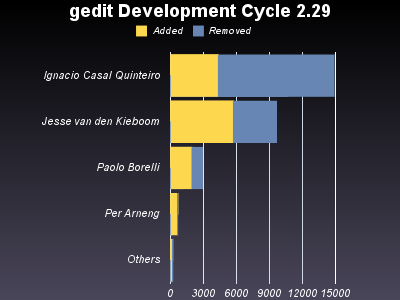
\includegraphics[scale=0.45]{./images/gedit-development-2-29}
    \caption{gedit development 2.29}
  \end{minipage}
  \hspace{0.5cm}
  \begin{minipage}[b]{0.5\linewidth}
    \centering
    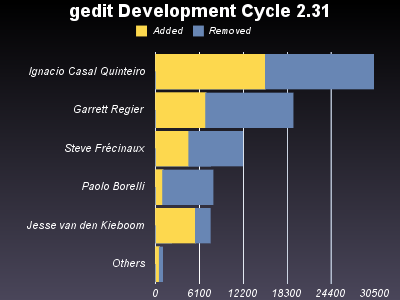
\includegraphics[scale=0.45]{./images/gedit-development-2-31}
    \caption{gedit development 2.31}
  \end{minipage}
\end{figure}

Just point out that this cycle has been particularly hard for application developers, especially those that try to adopt early, so that they are actually ready by the time GNOME 3.0 lands. And then to think, for the end user, there will be basiclly no change at all…

% mainfile:main.tex

\chapter{GNU General Public License}

\center{Version 2, June 1991}

\begin{center}
{\parindent 0in

Copyright \copyright\ 1989, 1991 Free Software Foundation, Inc.

\bigskip

51 Franklin Street, Fifth Floor, Boston, MA  02110-1301, USA

\bigskip

Everyone is permitted to copy and distribute verbatim copies
of this license document, but changing it is not allowed.
}
\end{center}

\begin{center}
{\bf\large Preamble}
\end{center}


The licenses for most software are designed to take away your freedom to
share and change it.  By contrast, the GNU General Public License is
intended to guarantee your freedom to share and change free software---to
make sure the software is free for all its users.  This General Public
License applies to most of the Free Software Foundation's software and to
any other program whose authors commit to using it.  (Some other Free
Software Foundation software is covered by the GNU Library General Public
License instead.)  You can apply it to your programs, too.

When we speak of free software, we are referring to freedom, not price.
Our General Public Licenses are designed to make sure that you have the
freedom to distribute copies of free software (and charge for this service
if you wish), that you receive source code or can get it if you want it,
that you can change the software or use pieces of it in new free programs;
and that you know you can do these things.

To protect your rights, we need to make restrictions that forbid anyone to
deny you these rights or to ask you to surrender the rights.  These
restrictions translate to certain responsibilities for you if you
distribute copies of the software, or if you modify it.

For example, if you distribute copies of such a program, whether gratis or
for a fee, you must give the recipients all the rights that you have.  You
must make sure that they, too, receive or can get the source code.  And
you must show them these terms so they know their rights.

We protect your rights with two steps: (1) copyright the software, and (2)
offer you this license which gives you legal permission to copy,
distribute and/or modify the software.

Also, for each author's protection and ours, we want to make certain that
everyone understands that there is no warranty for this free software.  If
the software is modified by someone else and passed on, we want its
recipients to know that what they have is not the original, so that any
problems introduced by others will not reflect on the original authors'
reputations.

Finally, any free program is threatened constantly by software patents.
We wish to avoid the danger that redistributors of a free program will
individually obtain patent licenses, in effect making the program
proprietary.  To prevent this, we have made it clear that any patent must
be licensed for everyone's free use or not licensed at all.

The precise terms and conditions for copying, distribution and
modification follow.

\begin{center}
{\Large \sc Terms and Conditions For Copying, Distribution and
  Modification}
\end{center}


%\renewcommand{\theenumi}{\alpha{enumi}}
\begin{enumerate}

\addtocounter{enumi}{-1}

\item 

This License applies to any program or other work which contains a notice
placed by the copyright holder saying it may be distributed under the
terms of this General Public License.  The ``Program'', below, refers to
any such program or work, and a ``work based on the Program'' means either
the Program or any derivative work under copyright law: that is to say, a
work containing the Program or a portion of it, either verbatim or with
modifications and/or translated into another language.  (Hereinafter,
translation is included without limitation in the term ``modification''.)
Each licensee is addressed as ``you''.

Activities other than copying, distribution and modification are not
covered by this License; they are outside its scope.  The act of
running the Program is not restricted, and the output from the Program
is covered only if its contents constitute a work based on the
Program (independent of having been made by running the Program).
Whether that is true depends on what the Program does.

\item You may copy and distribute verbatim copies of the Program's source
  code as you receive it, in any medium, provided that you conspicuously
  and appropriately publish on each copy an appropriate copyright notice
  and disclaimer of warranty; keep intact all the notices that refer to
  this License and to the absence of any warranty; and give any other
  recipients of the Program a copy of this License along with the Program.

You may charge a fee for the physical act of transferring a copy, and you
may at your option offer warranty protection in exchange for a fee.

\item

You may modify your copy or copies of the Program or any portion
of it, thus forming a work based on the Program, and copy and
distribute such modifications or work under the terms of Section 1
above, provided that you also meet all of these conditions:

\begin{enumerate}

\item 

You must cause the modified files to carry prominent notices stating that
you changed the files and the date of any change.

\item

You must cause any work that you distribute or publish, that in
whole or in part contains or is derived from the Program or any
part thereof, to be licensed as a whole at no charge to all third
parties under the terms of this License.

\item
If the modified program normally reads commands interactively
when run, you must cause it, when started running for such
interactive use in the most ordinary way, to print or display an
announcement including an appropriate copyright notice and a
notice that there is no warranty (or else, saying that you provide
a warranty) and that users may redistribute the program under
these conditions, and telling the user how to view a copy of this
License.  (Exception: if the Program itself is interactive but
does not normally print such an announcement, your work based on
the Program is not required to print an announcement.)

\end{enumerate}


These requirements apply to the modified work as a whole.  If
identifiable sections of that work are not derived from the Program,
and can be reasonably considered independent and separate works in
themselves, then this License, and its terms, do not apply to those
sections when you distribute them as separate works.  But when you
distribute the same sections as part of a whole which is a work based
on the Program, the distribution of the whole must be on the terms of
this License, whose permissions for other licensees extend to the
entire whole, and thus to each and every part regardless of who wrote it.

Thus, it is not the intent of this section to claim rights or contest
your rights to work written entirely by you; rather, the intent is to
exercise the right to control the distribution of derivative or
collective works based on the Program.

In addition, mere aggregation of another work not based on the Program
with the Program (or with a work based on the Program) on a volume of
a storage or distribution medium does not bring the other work under
the scope of this License.

\item
You may copy and distribute the Program (or a work based on it,
under Section 2) in object code or executable form under the terms of
Sections 1 and 2 above provided that you also do one of the following:

\begin{enumerate}

\item

Accompany it with the complete corresponding machine-readable
source code, which must be distributed under the terms of Sections
1 and 2 above on a medium customarily used for software interchange; or,

\item

Accompany it with a written offer, valid for at least three
years, to give any third party, for a charge no more than your
cost of physically performing source distribution, a complete
machine-readable copy of the corresponding source code, to be
distributed under the terms of Sections 1 and 2 above on a medium
customarily used for software interchange; or,

\item

Accompany it with the information you received as to the offer
to distribute corresponding source code.  (This alternative is
allowed only for noncommercial distribution and only if you
received the program in object code or executable form with such
an offer, in accord with Subsection b above.)

\end{enumerate}


The source code for a work means the preferred form of the work for
making modifications to it.  For an executable work, complete source
code means all the source code for all modules it contains, plus any
associated interface definition files, plus the scripts used to
control compilation and installation of the executable.  However, as a
special exception, the source code distributed need not include
anything that is normally distributed (in either source or binary
form) with the major components (compiler, kernel, and so on) of the
operating system on which the executable runs, unless that component
itself accompanies the executable.

If distribution of executable or object code is made by offering
access to copy from a designated place, then offering equivalent
access to copy the source code from the same place counts as
distribution of the source code, even though third parties are not
compelled to copy the source along with the object code.

\item
You may not copy, modify, sublicense, or distribute the Program
except as expressly provided under this License.  Any attempt
otherwise to copy, modify, sublicense or distribute the Program is
void, and will automatically terminate your rights under this License.
However, parties who have received copies, or rights, from you under
this License will not have their licenses terminated so long as such
parties remain in full compliance.

\item
You are not required to accept this License, since you have not
signed it.  However, nothing else grants you permission to modify or
distribute the Program or its derivative works.  These actions are
prohibited by law if you do not accept this License.  Therefore, by
modifying or distributing the Program (or any work based on the
Program), you indicate your acceptance of this License to do so, and
all its terms and conditions for copying, distributing or modifying
the Program or works based on it.

\item
Each time you redistribute the Program (or any work based on the
Program), the recipient automatically receives a license from the
original licensor to copy, distribute or modify the Program subject to
these terms and conditions.  You may not impose any further
restrictions on the recipients' exercise of the rights granted herein.
You are not responsible for enforcing compliance by third parties to
this License.

\item
If, as a consequence of a court judgment or allegation of patent
infringement or for any other reason (not limited to patent issues),
conditions are imposed on you (whether by court order, agreement or
otherwise) that contradict the conditions of this License, they do not
excuse you from the conditions of this License.  If you cannot
distribute so as to satisfy simultaneously your obligations under this
License and any other pertinent obligations, then as a consequence you
may not distribute the Program at all.  For example, if a patent
license would not permit royalty-free redistribution of the Program by
all those who receive copies directly or indirectly through you, then
the only way you could satisfy both it and this License would be to
refrain entirely from distribution of the Program.

If any portion of this section is held invalid or unenforceable under
any particular circumstance, the balance of the section is intended to
apply and the section as a whole is intended to apply in other
circumstances.

It is not the purpose of this section to induce you to infringe any
patents or other property right claims or to contest validity of any
such claims; this section has the sole purpose of protecting the
integrity of the free software distribution system, which is
implemented by public license practices.  Many people have made
generous contributions to the wide range of software distributed
through that system in reliance on consistent application of that
system; it is up to the author/donor to decide if he or she is willing
to distribute software through any other system and a licensee cannot
impose that choice.

This section is intended to make thoroughly clear what is believed to
be a consequence of the rest of this License.

\item
If the distribution and/or use of the Program is restricted in
certain countries either by patents or by copyrighted interfaces, the
original copyright holder who places the Program under this License
may add an explicit geographical distribution limitation excluding
those countries, so that distribution is permitted only in or among
countries not thus excluded.  In such case, this License incorporates
the limitation as if written in the body of this License.

\item
The Free Software Foundation may publish revised and/or new versions
of the General Public License from time to time.  Such new versions will
be similar in spirit to the present version, but may differ in detail to
address new problems or concerns.

Each version is given a distinguishing version number.  If the Program
specifies a version number of this License which applies to it and ``any
later version'', you have the option of following the terms and conditions
either of that version or of any later version published by the Free
Software Foundation.  If the Program does not specify a version number of
this License, you may choose any version ever published by the Free Software
Foundation.

\item
If you wish to incorporate parts of the Program into other free
programs whose distribution conditions are different, write to the author
to ask for permission.  For software which is copyrighted by the Free
Software Foundation, write to the Free Software Foundation; we sometimes
make exceptions for this.  Our decision will be guided by the two goals
of preserving the free status of all derivatives of our free software and
of promoting the sharing and reuse of software generally.

\begin{center}
{\Large\sc
No Warranty
}
\end{center}

\item
{\sc Because the program is licensed free of charge, there is no warranty
for the program, to the extent permitted by applicable law.  Except when
otherwise stated in writing the copyright holders and/or other parties
provide the program ``as is'' without warranty of any kind, either expressed
or implied, including, but not limited to, the implied warranties of
merchantability and fitness for a particular purpose.  The entire risk as
to the quality and performance of the program is with you.  Should the
program prove defective, you assume the cost of all necessary servicing,
repair or correction.}

\item
{\sc In no event unless required by applicable law or agreed to in writing
will any copyright holder, or any other party who may modify and/or
redistribute the program as permitted above, be liable to you for damages,
including any general, special, incidental or consequential damages arising
out of the use or inability to use the program (including but not limited
to loss of data or data being rendered inaccurate or losses sustained by
you or third parties or a failure of the program to operate with any other
programs), even if such holder or other party has been advised of the
possibility of such damages.}

\end{enumerate}


\begin{center}
{\Large\sc End of Terms and Conditions}
\end{center}


\pagebreak[2]

\section*{Appendix: How to Apply These Terms to Your New Programs}

If you develop a new program, and you want it to be of the greatest
possible use to the public, the best way to achieve this is to make it
free software which everyone can redistribute and change under these
terms.

  To do so, attach the following notices to the program.  It is safest to
  attach them to the start of each source file to most effectively convey
  the exclusion of warranty; and each file should have at least the
  ``copyright'' line and a pointer to where the full notice is found.

\begin{quote}
one line to give the program's name and a brief idea of what it does. \\
Copyright (C) yyyy  name of author \\

This program is free software; you can redistribute it and/or modify
it under the terms of the GNU General Public License as published by
the Free Software Foundation; either version 2 of the License, or
(at your option) any later version.

This program is distributed in the hope that it will be useful,
but WITHOUT ANY WARRANTY; without even the implied warranty of
MERCHANTABILITY or FITNESS FOR A PARTICULAR PURPOSE.  See the
GNU General Public License for more details.

You should have received a copy of the GNU General Public License
along with this program; if not, write to the Free Software
Foundation, Inc., 51 Franklin Street, Fifth Floor, Boston, MA  02110-1301, USA.
\end{quote}

Also add information on how to contact you by electronic and paper mail.

If the program is interactive, make it output a short notice like this
when it starts in an interactive mode:

\begin{quote}
Gnomovision version 69, Copyright (C) yyyy  name of author \\
Gnomovision comes with ABSOLUTELY NO WARRANTY; for details type `show w'. \\
This is free software, and you are welcome to redistribute it
under certain conditions; type `show c' for details.
\end{quote}


The hypothetical commands {\tt show w} and {\tt show c} should show the
appropriate parts of the General Public License.  Of course, the commands
you use may be called something other than {\tt show w} and {\tt show c};
they could even be mouse-clicks or menu items---whatever suits your
program.

You should also get your employer (if you work as a programmer) or your
school, if any, to sign a ``copyright disclaimer'' for the program, if
necessary.  Here is a sample; alter the names:

\begin{quote}
Yoyodyne, Inc., hereby disclaims all copyright interest in the program \\
`Gnomovision' (which makes passes at compilers) written by James Hacker. \\

signature of Ty Coon, 1 April 1989 \\
Ty Coon, President of Vice
\end{quote}


This General Public License does not permit incorporating your program
into proprietary programs.  If your program is a subroutine library, you
may consider it more useful to permit linking proprietary applications
with the library.  If this is what you want to do, use the GNU Library
General Public License instead of this License.



\nocite{*}
\bibliography{biblio}
\bibliographystyle{plain}

\end{document}
